
\documentclass[handout, 10pt,compress,xcolor={usenames,dvipsnames}]{beamer} %slides and notes
\usepackage{amsmath,datetime,xmpmulti,mathtools,bbm,mathabx,array,booktabs,alltt,xspace,tikz,calc,colortbl,graphicx}
\usepackage[usenames]{xcolor}
\usepackage[tikz]{mdframed}
\usepackage[author-year]{amsrefs}
\usepackage{newpxtext}
\usepackage[euler-digits,euler-hat-accent]{eulervm}
\usetikzlibrary{arrows}
\usepackage{cleveref}
\usepackage{multicol}
\usepackage{caption}
\usepackage{subcaption}
\usepackage{algorithm}
\usepackage{algorithmicx}% http://ctan.org/pkg/algorithm
\usepackage{algpseudocode}% http://ctan.org/pkg/algorithmicx
\usepackage{mathrsfs}


%%%%%
% Using Freds theme
%%%%%%%%%
\usetheme{FJHSlimNoFoot}


%%%%%
% Definitions from Freds Latex
%%%%%%%%%

\definecolor{ltred}{rgb}{0.75,0.8,0.75}

\setlength{\parskip}{2ex}
\setlength{\arraycolsep}{0.5ex}

\makeatletter
\newcommand{\vast}{\bBigg@{3}}
%\newcommand{\vast}{\bBigg@{4}}
\newcommand{\Vast}{\bBigg@{5}}
\makeatother


\title[]{Fast Automatic Bayesian Cubature \\ using Matching Kernels and Designs \\[1.0ex] }
\author[]{Jagadeeswaran R. \\
Adviser: Prof. Fred J Hickernell}
\institute{Department of Applied Mathematics,  Illinois Institute of Technology \\
	\href{mailto:jrathin1@iit.edu}{\url{jrathin1@iit.edu}} }
% \thanksnote{ Thanks to my employer Wi-Tronix for the trip sponsorship}
\date[]{Thesis Defense \textbullet\ Oct 22, 2019}
% \date[]{Computational Mathematics \& Statistics Seminar \textbullet\ Oct 11, 2019}

%% where the figures are stored
\graphicspath{{figures/}}
%\graphicspath{{./figures/}{/home/jagadees/MyWriteup/Sep_2ndweek/}}
%\graphicspath{{D:/Dropbox/writeup/BeamerPresent/}{D:/Dropbox/writeup/BeamerPresent/figures/}{D:/Mega/MyWriteupBackup/Sep_2ndweek/}}


\mdfdefinestyle{redshade}{%
	leftmargin=0 pt,
	rightmargin = 0pt,
	innerleftmargin = 1ex,
	innerrightmargin = 1ex,
	skipabove = 0 pt,
	skipbelow = 0 pt,
	backgroundcolor=red!20,
	linecolor=red!20,
	roundcorner=5pt}


\input FJHDef.tex
\newcommand{\bm}[1]{\boldsymbol{#1}}
\renewcommand{\mSigma}{\Sigma}
\renewcommand{\mLambda}{\Lambda}
\newcommand{\smallcite}[1]{{\small\cite{#1}}}
\newcommand{\smallocite}[1]{{\small\ocite{#1}}}
\newcommand{\smallcites}[1]{{\small\cites{#1}}}
\newcommand{\tol}{\text{tol}}
\newcommand{\Dt}{\text{D}}
\newcommand{\Ex}{\mathbb{E}}
\newcommand{\modop}[1]{{\left\lbrace{#1}\right\rbrace}}
\newcommand{\Ba}{\text{B}}
\newcommand{\hvtheta}{\hat{\vtheta}}

\newcommand{\MLE}{\textup{EB}}
\newcommand{\GCV}{\textup{GCV}}
\newcommand{\full}{\textup{full}}
\newcommand{\CI}{\textup{CI}}
\newcommand{\NICE}{\textup{NICE}}
\newcommand{\PEAKY}{{\textup{PEAKY}}}
\newcommand{\NOISE}{{\textup{NOISE}}}
\newcommand{\TRUE}{\textup{TRUE}}

\newcommand{\vC}{\bvec{C}}
\newcommand{\vW}{\bvec{W}}

\newcommand{\tvv}{\tilde{\vv}}

\newcommand{\mCtheta}{\mC_{\vtheta}}
\newcommand{\mCInv}{\mC^{-1}}
\newcommand{\mCthetaInv}{{\mathsf{C}^{-1}_{\vtheta}}}
\newcommand{\tmC}{\widetilde{\mC}}
\newcommand{\rmC}{\ring{\mC}}

\newcommand{\D}[1]{\text{d}{#1}}
\newcommand{\dvx}{\dif {\vx}}
\newcommand{\dvt}{\dif {\vt}}
\newcommand{\vthetaMLE}{{\vtheta}_{\MLE}}
\newcommand{\vrho}{\bm{\rho}}

\newcommand{\err}{{\text{err}}}
\newcommand{\errn}{{\text{err}}_{\text{n}}}
% \newcommand{\errtol}{{\text{err}}_{\text{tol}}}
% \newcommand{\errtol}{\text{tol}}
\newcommand{\errtol}{{\epsilon}}
\newcommand{\abstol}{{\text{err}}_{\text{abs}}}
\newcommand{\reltol}{{\text{err}}_{\text{rel}}}

\newcommand{\rlambda}{\ring{\lambda}}
\newcommand{\tmLambda}{\widetilde{\mLambda}}
\newcommand{\rmLambda}{\ring{\mLambda}}

\newcommand{\tB}{\widetilde{B}}
\newcommand{\tvC}{\widetilde{\vC}}
\newcommand{\rC}{\ring{C}}
\newcommand{\rvC}{\ring{\vC}}
\newcommand{\vPsi}{\bm{ \Psi}}
\renewcommand{\ty}{\widetilde{y}}
\renewcommand{\vtheta}{{\bm{\theta}}}
\newcommand{\vzeta}{{\bm{\zeta}}}



\newcommand{\pause}{}
\newtheorem{defn}{Definition}

\newcommand{\financePict}
{\href{http://i2.cdn.turner.com/money/dam/assets/130611131918-chicago-board-options-exchange-1024x576.jpg}
 {\includegraphics[height =
1.7cm]{130611131918-chicago-board-options-exchange-1024x576.jpg}}}

\newcommand{\GaussPict}
{\href{http://www.mathworks.com/matlabcentral/answers/uploaded_files/26298/Plotting\%20a\%203d\%20gaussian\%20function\%20using\%20surf\%20-\%202015\%2002\%2027.png}
 {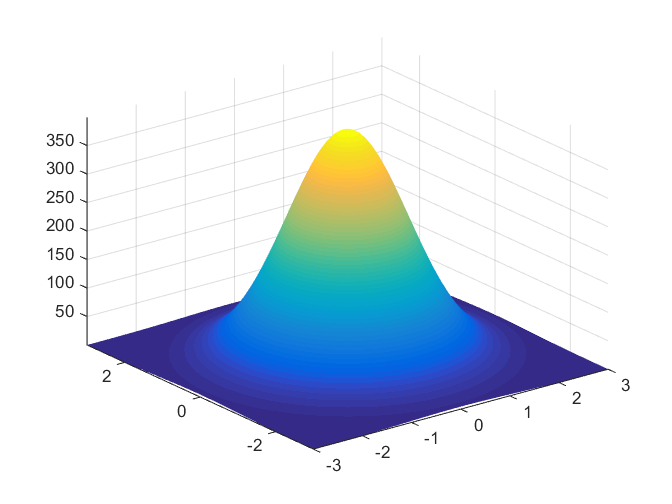
\includegraphics[height
 = 2cm]{../figures/Plotting_gaussian.png}}}

\DeclareMathOperator{\Var}{VAR}
\DeclareMathOperator{\disc}{DSC}
\DeclareMathOperator{\algn}{ALN}
%\DeclareMathOperator{\GP}{\cg\cp}

\newcommand{\redroundmathbox}[1]{\parbox{\widthof{$#1$\hspace{1em}}}
	{\begin{mdframed}[style=redshade]\centering $#1$ \end{mdframed}}}
\newcommand{\setbeameruncoveredtransp}{\setbeamercovered{transparent=10}}

\def\abs#1{\ensuremath{\left \lvert #1 \right \rvert}}


\makeatletter
\patchcmd{\beamer@sectionintoc}
  %{\vfill}
  {\vskip\itemsep}
  %{}
  %{}
\makeatother

\algdef{SE}[DOWHILE]{Do}{doWhile}{\algorithmicdo}[1]{\algorithmicwhile\ #1}%



\begin{document}
\tikzstyle{every picture}+=[remember picture]
\everymath{\displaystyle}


\frame{\titlepage}







\iftrue
%\frame{\frametitle{Table of contents}\tableofcontents}
\begin{frame}{\contentsname}
    \begin{minipage}{\textwidth}
    	\vspace{-6ex}
		\linespread{1.4}
		\begin{multicols}{2}
			% \tableofcontents
			\tableofcontents[subsectionstyle=hide] %\tableofcontents		
		\end{multicols}
    \end{minipage}
	\addtocounter{framenumber}{-1}% If you don't want them to affect the slide number
\end{frame}
\fi


\iffalse
\AtBeginSection[]
{
	\begin{frame}
		\begin{minipage}{\textwidth}
		\frametitle{Outline}
		\vspace{-6ex}
		\linespread{2}
		\begin{multicols}{2}
			\tableofcontents[currentsection,subsectionstyle=hide] %\tableofcontents
		\end{multicols}
		\end{minipage}
	\addtocounter{framenumber}{-1}% If you don't want them to affect the slide number
	\end{frame}
}
\fi 




\section{Introduction}
\frame
{
\frametitle{Numerical Integration}
\vspace{-5ex}
A fundamental problem in various fields, including finance, machine learning and statistics:
\vspace{-2ex}
\begin{align}
\label{eqn:defn_mu}
\mu = \int_{\reals^d} g(\vx) \,  \dif \vx = \int_{[0,1]^d} f(\vx) \,
\dif\vx  = & \Ex[f(\vX)] = ?, \quad \text{where} \quad \vX \sim \cu [0,1]^d
\end{align}
\vspace{-5ex}
\begin{align*}
 &\text{Use a cubature} \quad
\hmu_n := w_0 + \sum_{j=1}^{n} f(\vx_j) w_j \qquad
\\  \vspace{-2ex}
& \qquad \text{with points $\{\vx_j \}_{j=1}^{n}$ and associated weights $w_j$.}
\end{align*}
\vspace{-1ex}
\pause %using  points $\{\vx_j \}_{j=1}^{n}$ and associated weights $w_j$.
The goal of this work is to
\vspace{-2ex}
\begin{itemize}
\item Develop an automatic algorithm for integration
\item Use an \alert{extensible} point-set and an algorithm that allows extending points 
\item Determine \alert{$n$} such that, given \alert{$\errtol$}, $\abs{\mu-\hmu_n} \leq \errtol$
\end{itemize}
}








\begin{frame}{Bayesian Cubature}
	% Deterministic or Random
	\vspace*{-4ex}
	Bayesian approach for numerical analysis popularized by \ocite{Dia88a}; 
	interpreted trapezoidal rule, splines, and other methods from the statistical point of view.
	%For example, the trapezoidal rule can be interpreted as a Bayesian 	method with prior information being modeled as a Brownian motion in the sample 	space $C[0, 1)$, the space of continuous functions.
	
	% Bayesian approach for numerical integration that is known as Bayesian cubature as introduced by \ocite{OHa91a}.
	See also \ocite{OHa91a}.
	
	
	% The Bayesian approach for numerical analysis was popularized by Diaconis [7].
	% The earliest reference for such kind of approach dates back to Poincar'e, where, the theory of interpolation was discussed. Diaconis motivates the reader by interpreting the most well known numerical methods, 1) trapezoidal rule and 2) splines, from the statistical point of view with whatever is known about the integrand as prior 	information. For example, the trapezoidal rule can be interpreted as a Bayesian 	method with prior information being modeled as a Brownian motion in the sample 	space C[0; 1), the space of continuous functions.
	
	\begin{itemize}
		\item Assume \alert{$f$} is drawn from a Gaussian process 
		\begin{itemize}
			\item Need to estimate the mean and covariance kernel
		\end{itemize}
		\item Parameter estimation (Empirical Bayes, Cross validation) is expensive in general
		\begin{itemize}
			\item Use points and kernel for which it is cheap
		\end{itemize}
	\end{itemize}

	% \uncover<2>
	{
	\textbf{Problem:}
	\vspace*{-4ex}
	\begin{itemize}
		\item How to choose \alert{$\{\vx_i\}_{i=1}^n$}, and
		\alert{$\{w_i\}_{i=1}^n$} to make $\abs{\mu - \hmu_n}$ small? How to estimate credible interval $\err_\CI$? 
		\alert{(Bayesian posterior error)}
		\item How to find $n$ such that $\abs{\mu - \hmu_n} \le \err_\CI \le \errtol $ ? \alert{(automatic cubature)}
	\end{itemize}
}
\end{frame}




































\section{Bayesian Cubature}


\subsection{Posterior Error}


\begin{frame}
\frametitle{Bayesian posterior error}
\vspace*{-4ex}
\alert{Assume random}
$f \sim \mathcal{GP} (m, s^2C_{\vtheta})$,
a \alert{Gaussian process} with mean $m$ and covariance kernel $s^2C_{\vtheta}$, $C_{\vtheta}:[0,1]^d \times [0,1]^d \to \reals$ .
\vspace*{-1ex}
\begin{align*}
\text{Define} \quad c_{0,\vtheta} &= \int_{[0,1]^d \times [0,1]^d} C_{\vtheta} (\vx,\vt) \dvx \dvt, 
\\
\vc_{\vtheta}& = \left( \int_{[0,1]^d } C_{\vtheta} (\vx_i,\vt) \dvt \right)_{i=1}^n,
\quad
\mCtheta =  \biggl( C_{\vtheta} (\vx_i,\vx_j) \biggr)_{i,j=1}^n
\end{align*}
\pause
\vspace*{-3ex}
\begin{align*}
\mu - \hmu_n  \big \vert \vy & \; \sim \;
\cn
\biggl( %-w_0 + m(1- \bm{1}^T \mCthetaInv\vc) + \vy^T (\mCthetaInv\vc - \vw)
0, \quad s^2(c_{0,\vtheta} - \vc_{\vtheta} ^T \mCthetaInv \vc_{\vtheta})
\biggr)
\quad % \\
\text{where} \; \vy = \bigl(f(\vx_i)\bigr)_{i=1}^n. 
\\
\text{Choosing} \; \hmu_n &= \underbrace{m(1 - \vone^T \mCthetaInv \vc_{\vtheta})}_{w_0} + {(\underbrace{\mCthetaInv \vc_{\vtheta}}_{\vw})}^T \vy \; \text{makes error unbiased.} 
\end{align*}
\pause
If $\alert{m = 0}$, fixed, choosing $\vw = \mCthetaInv\vc_{\vtheta} \;$ makes error unbiased. Please note \alert{$m, s$ and $\vtheta$} needs to be inferred.

\ocite{Dia88a}, \ocite{OHa91a}, \ocite{Rit00a}, \ocite{RasGha03a}, \ocite{BriEtal18a}, \ocite{TraWasWoz88} and others
\end{frame}







\subsection{Parameter estimation}

%\subsection{Empirical Bayes}


\begin{frame}
\frametitle{Parameter estimation - Empirical Bayes}
\vspace*{-5ex}
Maximize the log-likelihood of the parameters given the data $\vy = (f(\vx_i))_{i=1}^{n}$ w.r.t. $m$ then $s^2$, then with $\vtheta$: 
\begin{align*}
m_{\MLE} &= \frac{\bm{1}^T \mCthetaInv \vy}{\bm{1}^T \mCthetaInv \bm{1}}, & \text{(Explicit)} 
\\
%s^2_{\MLE} &= \frac{1}{n} (\vy-m_{\MLE}\bm{1})^T \mCthetaInv (\vy-m_{\MLE}\bm{1})  , & \text{(Explicit)} \\
s^2_{\MLE} 
&= 
\frac{1}{n}
\vy^T 
\left[ \mCthetaInv - 
\frac{ \mCthetaInv \vone \vone^T \mCthetaInv }{\vone^T\mCthetaInv \vone}
\right] \vy, & \text{(Explicit)} 
\\
\vthetaMLE &= \argmin_{\vtheta}
\log
\left(
\frac{1}{2n} \log(\det \mCtheta) + \log(s_\MLE)
\right)
 & \text{(numeric)}
\\
\hmu_\MLE  &= 
\left(
\frac{ (1 - \vone^T  \mCthetaInv\vc_{\vtheta} )  \vone }{ \vone^T \mCthetaInv \vone}   +  \vc_{\vtheta} 
\right)^T  \mCthetaInv \vy  , & \text{(Explicit)} 
\intertext{The credible interval width, $\err_{\MLE}$, is given by}
\err_{\MLE} & = 2.58 \; s_{\MLE} \; \sqrt{c_{0,\vtheta} - \vc_{\vtheta}^T\mCthetaInv\vc_{\vtheta} }, \quad \vtheta = \vtheta_\MLE
\end{align*}
\pause %\vspace{-3ex}
% \alert{Why do we need $\vtheta_{\MLE}$?} \quad The sample space spanned by $C_{\vtheta}$ customized to have the integrand $f$ in the middle.
Computational cost \alert{ $\Order\bigl(n \$(f) + N_{\opt}[n^2\$(C_\vtheta) + n^3] \bigr)$}.
\end{frame}






\iffalse

\subsection{Bayesian cubature : Summary}


\frame{
\frametitle{Bayesian cubature using MLE results : Summary}
\vspace{-8ex}
\begin{align*}
\text{Assume}  \; f &\sim \mathcal{GP} (m, s^2 C_{\vtheta}) \; \text{given} \;
\vy =\bigl( f(\vx_i) \bigr)_{i=1}^{n},
\\
\mu - \hmu_n & \big \vert \vy
\; \sim \;
\cn
\bigl(w_0 +
m(1- \bm{1}^T \mCthetaInv\vc) +
\vy^T (\mCthetaInv\vc - \vw), \quad s^2(c_0 - \vc ^T \mCthetaInv \vc)
\bigr)
\end{align*}
\pause
\vspace{-4ex}
\begin{align*}
\;  m_\MLE = \frac{\bm{1}^T \mCthetaInv \vy}{\bm{1}^T \mCthetaInv \bm{1}},& \; \text{and} \; \quad
s^2_\MLE = \frac {1}{n} \vy^T
\left[ \mCthetaInv - \frac{\mCthetaInv \vone \vone^T \mCthetaInv}{\vone^T \mCthetaInv \vone}\right] \vy,
\\
\vthetaMLE &= \argmin_{\vtheta}
\log
\left[
\frac{1}{2n} \log(\det \mC) + \log(s_\MLE)
\right]
\\
 \;
\hmu_n &=  w_0 +  \vw^T \vy =
m_\MLE
(1 - \bm{1}^T \mCthetaInv \vc)
+ \vc^T\mCthetaInv \vy,
\\
\mathbb{P}[\lvert\mu - \hat{\mu}_n\rvert \le \text{err}_n] & \geq  99\% ,
\\
\text{If} \quad
\text{err}_n & \leq 2.58 \; s_\MLE \; \sqrt{\bigl (c_{0} - \vc^T  \mCthetaInv \vc \bigr)}
\\
& \text{Where $c_0$, $\vc$ and $\mC$ depend on $\vthetaMLE$}
\end{align*}
\pause
\alert{Problem :} 
\\
$\mCthetaInv$ typically requires \alert{$\Order(n^3)$} operations, which makes it impractical for large $n$.
}
\fi

























\iffalse

\frame{
\frametitle{Bayesian Cubature - Deterministic Interpretation}
\vspace{-7.8ex}
\begin{align*}
f \in & \cf \text{ with reproducing kernel } C_{\vtheta}
\\
\text{if }  &
\Var^{\Dt}(f - \tf_{\vy}) \le \frac{2.58}{\alert{\sqrt{n}}} \Var^{\Dt}(\tf_{\vy})
\end{align*}
\pause
\begin{align*}
\text{\alert{replace} } & C_{\vtheta} \text{ by } C_{\vtheta}
\\
\text{err}_n &= 2.58 \disc^{\Ba}(\nu - \hnu) \Var^{\Ba}(f)
\\
\vthetaMLE &= \argmin_{\vtheta}  \vol \bigl(\bigl( \vz \in \reals^n :
\quad \Var^{\Dt}_{\vtheta}(\tf_{\vz}) \le \Var^{\Dt}_{\vtheta}(\tf_{\vy}) \bigr) \bigr ) \\
\tf_{\vy}: & \; \text{minimum norm interpolant}
\end{align*}


}
\fi






\iffalse
\begin{frame}<1>[label=BayesCub]
\setbeameruncoveredtransp
\frametitle{Bayesian Cubature \hfill \uncover<2->{Deterministic Interpretation}}
\vspace{-7.8ex}
\[
\begin{array}{rcl}
f  \sim \mathcal{GP} (0, s^2 C_{\vtheta})
&
&
\uncover<2->{f \in \cf \text{ w/ reproducing kernel } C_{\vtheta}}
\tabularnewline
\toprule
\multicolumn{3}{c}{\abs{\mu - \hmu} \le \text{ width}}
\tabularnewline
\text{with } 99\% \text{ confidence}
&
&
\uncover<3->{\text{if }
\Var^{\Dt}(f - \tf_{\vy}) \le \frac{2.58}{\alert{\sqrt{n}}} \Var^{\Dt}(\tf_{\vy}) }\tabularnewline
2.58\sqrt{\bigl (c_{\vthetaMLE,0} - \vc_{\vthetaMLE}^T  \mC_{\vthetaMLE}^{-1} \vc_{\vthetaMLE}\bigr) \, \frac {\vy^T \mC_{\vthetaMLE}^{-1}  \vy}{\alert{n}} }
&
\shortleftarrow\text{\!width}\uncover<2->{\!\shortrightarrow}
&
\uncover<2->{\text{\alert<2>{replace} } C_{\vtheta} \text{ by } C_{\vtheta}}
\tabularnewline
= 2.58 \disc^{\Ba}(\nu - \hnu) \Var^{\Ba}(f)
&
&  \uncover<3->{=\frac{2.58}{\alert{\sqrt{n}}}\disc^{\Dt}(\nu - \hnu) \Var^{\Dt}(\alert{\tf_{\vy}}) }
\tabularnewline
\multicolumn{3}{c}{\vy = \bigl(f(\vx_i)\bigr)_{i=0}^{n-1}}
\tabularnewline[0.5ex]
&
&
\uncover<3->{\tf_{\vy} = \text{minimum norm interpolant}}
\tabularnewline
\mC_{\vthetaMLE}^{-1} \vc_{\vthetaMLE} & \leftarrow \vw \uncover<2->{\rightarrow}
&
\uncover<2->{\text{\alert<2>{replace} } C_{\vtheta} \text{ by } C_{\vtheta}}
\tabularnewline
\argmin_{\vtheta} \frac{\vy^T \mC_{\vtheta}^{-1} \vy}{[\det(\mC_{\vtheta}^{-1})]^{1/n}}
&
\leftarrow 	\vthetaMLE  \uncover<2->{\rightarrow}
&
\uncover<2->{\text{\alert<2>{replace} } C_{\vtheta} \text{ by } C_{\vtheta}}
\tabularnewline
\text{estimate $s$ and $\vtheta$ by MLE}
&
&
\uncover<3->{ = \argmin_{\vtheta}  \vol \bigl(\bigl( \vz \in \reals^n :
\tabularnewline
&
&
\qquad\quad \Var^{\Dt}_{\vtheta}(\tf_{\vz}) \le \Var^{\Dt}_{\vtheta}(\tf_{\vy}) \bigr) \bigr ) }
\end{array}
\]
\iffalse
\only<1>{\qquad \alert{Nice:\quad}$
\begin{array}{c@{\quad}ccccc}
\vy, \, \mC_{\vtheta} & \vw & \hmu & \text{width}& \vthetaMLE  \tabularnewline
\toprule
47 \vy, \, 29 \mC_{\vtheta} & \vw & 47 \hmu & 47 \text{width} & \vthetaMLE
\end{array}$}
\fi
\only<3->{%
\\[-1ex]
%		\begin{tabular}{m{2.4cm}@{}m{9.2cm}}
%	\quad \alert{Unfortunately: }  &
\begin{itemize}\setlength{\itemsep}{-0.3ex}
\item Requires $\Order(n^3)$ operations to compute $\mC_{\vtheta}^{-1}$, but see \smallocite{AniCheSte16a}
\item Ill-conditioning for smoother kernels (faster convergence)
\item Might not integrate constants exactly
\end{itemize}
%\end{tabular}
}

\end{frame}
\fi




\subsection{Automatic cubature algorithm}

\frame{
	% \setbeameruncoveredtransp
	%\frametitle{Algorithm }
	\vspace*{-6ex}
	% \uncover<1-2>
	{
		\begin{algorithm}[H]
			\begin{algorithmic}[1]
				\Procedure{AutoBayesCubature}{$f$,$\errtol$} 
				%\Comment{Integrate within the error tolerance \alert{$\errtol$}}
				\Require a generator for the sequence
				$\vx_1, \vx_2, \ldots$; 
				a black-box function, $f$; 
				an absolute error tolerance,
				$\varepsilon>0$; the positive initial sample size, $n_0$;
				the maximum sample size $n_{\textup{max}}$
				% \State $n_0 \gets 2^8$ \Comment{start with minimum number of points}
				\State $n\gets n_0, \; n' \gets 0, \; \err_\CI \gets \infty$
				%\Do
				\While{$\err_\CI > \varepsilon$ and $n \le n_{\textup{max}}$} %\Comment{Iterate till error tolerance is met}
				\State Generate $\{ \vx_i\}_{i=n' + 1}^{n}$ and sample $\{f(\vx_i)\}_{i=n'+1}^{n}$, 
				\State Compute parameters, % $\vtheta$, 
				compute error bound \alert{$\err_\CI$ } %\Comment{$\errn$ data driven error bound}
				%\If{\alert{$\errn \leq \errtol$}}
				%    \textbf{break}
				%\EndIf
				\State $n' \gets n, \; n\gets 2 \times n'$
				\EndWhile
				\State Sample size to compute $\hmu$, $n \gets n'$
				% \State Compute cubature weights $\{ w_i \}_{i=1}^{n}$
				\State Compute approximate $\hmu_n$, the approximate integral
				\State \textbf{return} $\hmu_n$ \Comment{Integral estimate $\hmu_n$}
				\EndProcedure
			\end{algorithmic}
			%\caption{Template}\label{algorithmBasic}
	\end{algorithm}}
	%\vspace*{-4.5ex}

}





\subsection{Example with Mat\'ern  kernel}
\begin{frame}
\frametitle{Multivariate Gaussian integration with Mat\'ern kernel}
\vspace{-8ex}
\begin{align}
\label{eqn:matern_kernel_order_3by2}
\text{Mat\'ern covariance kernel:} \; C_{\theta}(\vx, \vt) = \prod_{\ell=1}^d \exp(-\theta|\vx_\ell-\vt_\ell|)(1+\theta |\vx_\ell-\vt_\ell|) %\\
%\text{Multivariate Gaussian:} \; 
%\label{eqn:GaussDef}
%\mu = \int_{(\va,\vb)} \frac{\exp\bigl(- \frac 12 \vt^T \mSigma^{-1} \vt \bigr)}{\sqrt{(2 \pi)^d \det(\mSigma)}} \, \dvt.
\end{align}
\begin{equation*}
d = 3, \quad \va = \begin{pmatrix}
-6 \\ -2 \\ -2
\end{pmatrix}, \quad 
\vb = \begin{pmatrix}
5 \\ 2 \\ 1
\end{pmatrix} , \quad 
\mL = \begin{pmatrix}
4 & 1 & 1 \\ 0 & 1 & 0.5 \\ 0 & 0 & 0.25
\end{pmatrix}.
\end{equation*}

\vspace{-3ex}

\begin{figure}[htp]
\captionsetup[subfigure]{labelformat=empty}
\centering
\begin{subfigure}[b]{0.49\textwidth}
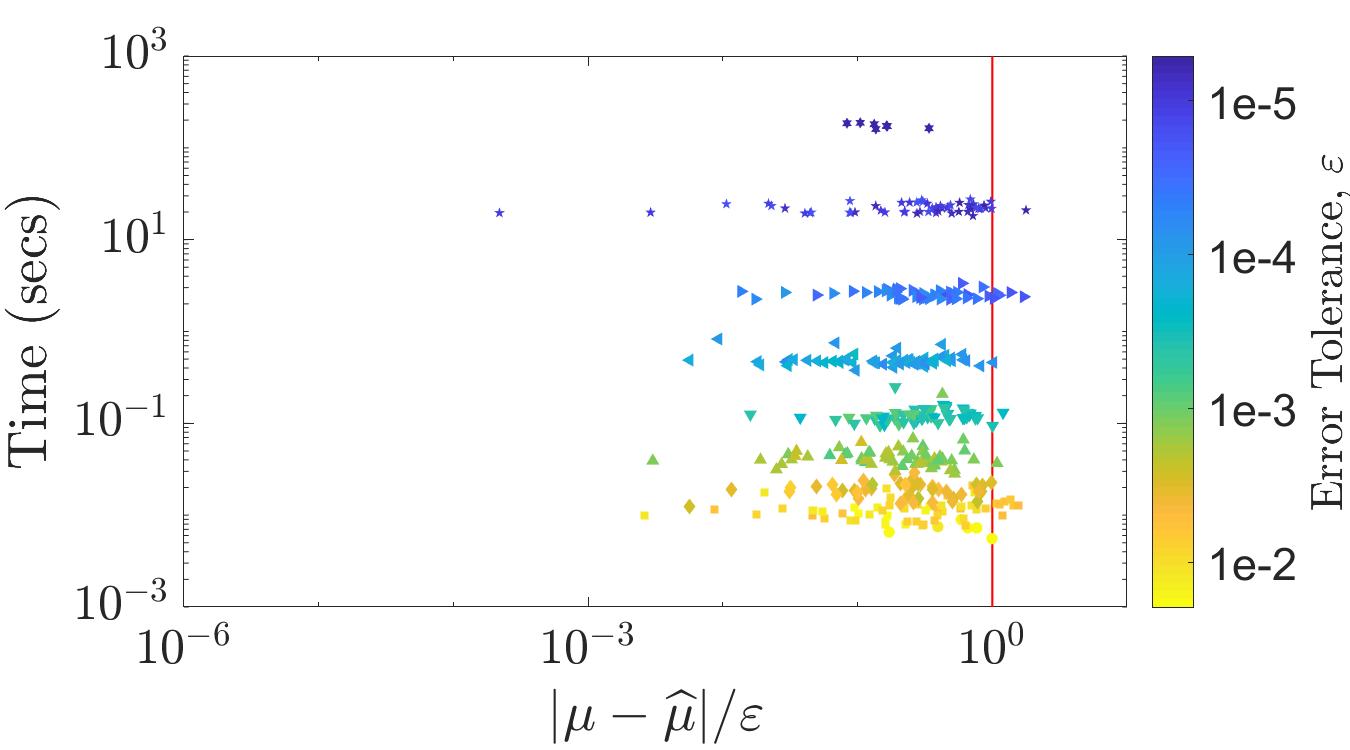
\includegraphics[height=3.25cm]{../figures/MVN_guaranteed_time_Matern_d2_2019-Jun-29}
\end{subfigure}
\centering
\begin{subfigure}[b]{0.49\textwidth}
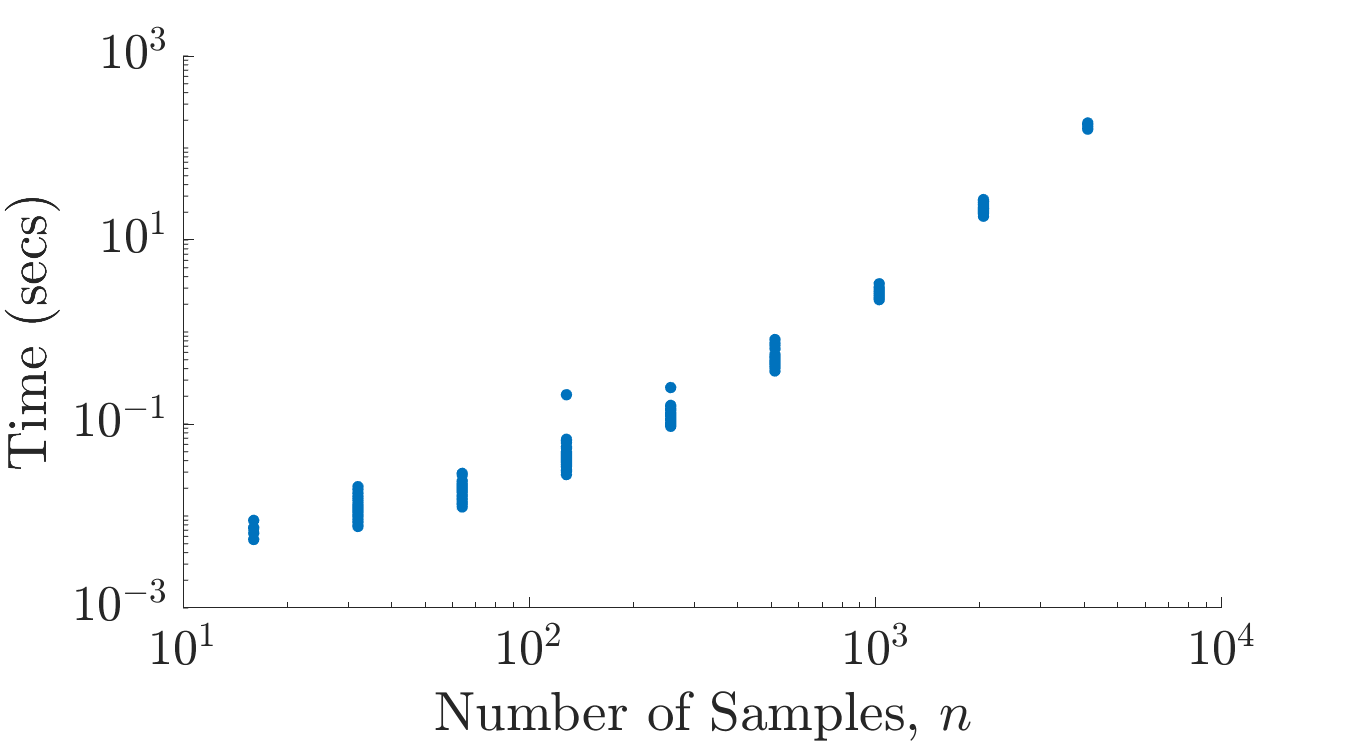
\includegraphics[height=3.25cm]{../figures/MVN_rapid_n_vs_time_Matern_d2_2019-Jun-29}
\end{subfigure}
%\caption{  }
\label{fig:MVN_Metern_d2b2}
\end{figure}
\alert{Problem}: Computation time (in seconds) increases rapidly, so it is not practical to use more than 4000 points in the cubature.
\end{frame}
















\section{Faster}



\subsection{Fast Bayesian Transform}



\begin{frame}
\frametitle{Fast Bayesian Transform}
\vspace{-4ex}
Choose the kernel $C_{\vtheta}$ and $\{\vx_i\}_{i=1}^n$, so the Gram matrix $\mCtheta =  \left( C_{\vtheta} (\vx_i,\vx_j) \right)_{i,j=1}^n$ has:
\vspace{-2ex}
\begin{align*}
\mCtheta =& (\vC_1,...,\vC_n)
=  \frac 1n \mV \mLambda \mV^H, \quad
\mV = (\vV_1,...,\vV_n) = (\vv_1,...,\vv_n)^T
\end{align*}
\pause 
\vspace{-2ex}
$C_{\vtheta}$ is a fast Bayesian transform kernel, if,
\begin{enumerate}
	\item $\mV$ { may be identified analytically}
	\item $\vv_1 = \vV_1 = \vone$
	\item \alert{Computing $\widetilde{\vb} = \mV^H \vb$ requires only $\Order(n \log n)$ operations  $\forall \vb$.}
\end{enumerate}
\vspace{-1.5ex}
The covariance kernel may also be normalized 
\begin{align*}
%\label{addAssump}
\int_{[0,1]^d} C_\vtheta(\vt,\vx) \, \D \vt = 1 \qquad \forall \vx \in [0,1]^d,
\text{ leading to $c_{0,\vtheta} = 1$ and $\vc_{\vtheta} = \vone$}.
\end{align*}
Please note that
\begin{align*}
\mLambda &= \diag (\vlambda), \quad \vlambda = (\lambda_1,...,\lambda_n) = \mV^H \vC_1.
\end{align*}

\end{frame}











\iffalse
\begin{frame}
\frametitle{Fast transform kernel --- More detailed}
\vspace{-5ex}
Choose the kernel $C_{\vtheta}$ and $\{\vx_i\}_{i=1}^n$ so the Gram matrix $\mC =  \left( C_{\vtheta} (\vx_i,\vx_j) \right)_{i,j=1}^n$ has the special properties
\vspace{-2ex}
\[
\begin{array}{lcc}
\quad
\mC =  \frac 1n \mV \mLambda \mV^H =  \frac 1n \mV^* \mLambda \mV^T = \mC^T,
\quad \quad
\mCthetaInv = \frac 1n \mV \mLambda^{-1} \mV^H = \frac 1n \mV^* \mLambda \mV^T,
\\
\mV := (\vv_1,...,\vv_n)^T = (\vV_1,...,\vV_n), \quad
\vV_1 = \vv_1 := \vone, \quad \mLambda = \diag (\lambda_1,...,\lambda_n)
\\ \pause
\\
\quad \quad
\mC \vone = \lambda_1 \vone, \quad \mCthetaInv \vone= \frac{1}{\lambda_1} \vone,
\quad \quad
\sum_{j=1}^n C(\vx_i, \vx_j) = \lambda_1, \; \forall i = 1,...,n,
\\
\mV^H = n \mV^{-1}, \quad \quad
\mV^H  \mV  = n
=
\mV^T \mV^* , \quad \quad c_0 := 1 \quad  \vc := \vone
\\ \pause
\\
\text{If} \quad
\mC = (\vC_1,...,\vC_n), \text{then}
\\
\mV^T \vC_1 = \mV^T \left( \frac 1n \mV^* \mLambda \vv_1 \right) =
\underbrace{\left( \frac 1n \mV^T  \mV^* \right) }_{I} \mLambda \vv_1  =  \mLambda \vone =
\begin{pmatrix}
\lambda_1 \\ \vdots \\ \lambda_n
\end{pmatrix}
\\
\text{A fast trasnform kernel $C_{\vtheta}$ is for which the transform }
{
\redroundmathbox{
{
\text{$\hat{\vz} = \mV^T \vz$ }
 } } }
\\
\text{can be done in $\Order( n \, log\, n) $}
\end{array}
\]
\end{frame}
\fi









\subsection{Shape parameter $\vthetaMLE$ and Error Bound}

\begin{frame}
	{Computing the $\vtheta$, $\err_{\CI}$, and $\hmu$ faster}
\vspace{-9ex}
%Using the properties of the \alert{fast Bayesian transform}, the estimates of $\vtheta$ and the error bound \alert{$\errn$} can be computed faster:
\vspace{-1ex}
\begin{subequations}
%\label{thetaSimple}
\begin{align*}
\vthetaMLE &= 
\argmin_{\theta} \left[ \log\left(  \sum_{\alert{i=2}}^{n} \frac{|\ty_i|^2}{\lambda_i} \right) + \frac{1}{n}\sum_{i=1}^{n} \log( \lambda_i ) \right]
\\
\vtheta_{\GCV} 
&= \argmin_{\vtheta} \left[ \log \left ( \sum_{\alert{i=2}}^n \frac{\abs{\ty_i}^2}{\lambda_i^{\alert{2}}} 
\right) -2\log\left( \sum_{i=1}^n \frac{1}{\lambda_i} \right)
\right]
\end{align*}
\end{subequations}
\vspace{-5ex}
\begin{subequations}
%\label{fastStoppingCriterions}
\begin{align*}
\err_{\MLE} = 
\frac{2.58}{n} &\left\{ \sum_{\alert{i=2}}^{n} \frac{\abs{\ty_i}^2}{\lambda_i}  
\left( 1 - \frac{n}{\lambda_1} \right)\right\}^{1/2}
\\
\err_{\full}
=
\frac{t_{n-1,0.995}}{n} &
\left\{\frac{\lambda_1}{(n-1)} \sum_{\alert{i=2}}^n \frac{\abs{\ty_i}^2}{\lambda_i} \, \left(1 - \frac{n}{\lambda_1}  \right)\right\}^{1/2}
\\
\err_{\GCV}  =
\frac{2.58}{n} &
\left\{\sum_{\alert{i=2}}^n \frac{\abs{\ty_i}^2}{\lambda_i^{\alert{2}}}  \left [ \frac 1n \sum_{i=1}^n \frac{1}{\lambda_i} \right]^{-1}  \times
\left( 1 -  \frac{n}{\lambda_1} \right)  
\right\}^{1/2}
\end{align*}
\end{subequations}
\vspace{-4ex}
Similarly, \alert{$\hmu$} can be computed faster
$ \hmu_\MLE = \hmu_{\full} = \hmu_\GCV = 
\redroundmathbox{
{ \frac1n \sum_{i=1}^n {{y}_i} } }$
%  where $\tvy = \mV^T \vy, \quad   \vlambda =  \mV^T \vC_1, \; \vC_1 = \left( C(\vx_i, \vx_1) \right)_{i=1}^{n} $
% \alert{$\Order(n )$ operations to compute the $\hmu$}. \alert{$\Order(n \log n)$ operations to compute $\tvy$ and $\hat{\vlambda}$, So the $\vthetaMLE$ and $\err$}
\end{frame}




\begin{frame}{Fast Bayesian Transform}
	\redroundmathbox{
\text{Computational cost} \quad { \Order\bigl(n \$(f) + N_{\opt}[n\$(C_\vtheta) + n \log{n} ] \bigr)}.}
\end{frame}




\iffalse

\subsection{Algorithm - Bayesian Cubature}
\frame{
\frametitle{Automatic Bayesian Cubature}
\begin{algorithm}[H]
  \caption{Automatic Bayesian Cubature}\label{algorithm}
  \begin{algorithmic}[1]
    \Procedure{BayesCubature}{$f,\text{err}_{tol}$} \Comment{Integrate within the error threshold}
      \State $n \gets 2^8$
      \Do
        \State Generate Lattice points$(\vx_i)_{i=0}^{n-1}$
        \State Sample $(f(\vx_i))_{i=0}^{n-1}$
        \State Estimate optimal params $\vthetaMLE_n$
        \State Compute $\mathsf{C}_{\vthetaMLE, n}$
        \State Compute $\text{err}_{n}$
        \State $n\gets 2 \times n$
      \doWhile{$\text{err}_{n} > \text{err}_{tol}$}   \Comment{Iterate till error tolerance is met}
      \State Compute weights $(w_i)_{i=0}^{n-1}$
      \State Compute $\hmu_n$
      \State \textbf{return} $\hmu_n$ \Comment{Integral estimate $\hmu_n$}
    \EndProcedure
  \end{algorithmic}
\end{algorithm}
}

\fi







\iffalse
\begin{align*}
\text{Baker} & : & \tf(\vt)
= f\left(1-2|\vt-\frac{1}{2}| \right)
\\
\text{C0} & : & \tf(\vt)
= f\left(3\vt^2 - 2\vt^3\right)\prod_{j=1}^d(6t_j(1-t_j))
\\
\text{C1} & : & \tf(\vt)
= f\left(\vt^3(10-15\vt+6\vt^2)\right)\prod_{j=1}^d(30t_j^2(1-t_j)^2)
\\
\text{Sidi's C1} & : & \tf(\vt)
= f\left( \left( t_j- \frac{\sin(2\pi t_j)}{2\pi} \right)_{j=1}^d \right)\prod_{j=1}^d(1-\cos(2\pi t_j))
\end{align*}

%varies in terms of computational complexity and accuracy, choose based on the smoothness of the integrand.

\begin{enumerate}
\item Baker : Baker's transform or tent map in each coordinate. It preserves only continuity but it is easier to compute.
\item C0 : polynomial transformation only preserving continuity.
\item C1 : polynomial transformation preserving the first derivative.
\item C1sin : Sidi's transform with Sine, preserving the first derivative. This is in general a better option than 'C1'.
\end{enumerate}
\fi

































\section{Lattice Nodes}


%\subsection{Lattice nodes and shift invariant covariance kernels}
\subsection{Shift invariant covariance kernels}













\subsection{Rank-1 Lattice points}
\frame{ \frametitle{Rank-1 Lattice rules : low discrepancy point set }
\vspace{-5ex}
\only<1>{
Given the \alert{generating vector $\vh$}, the construction of \alert{n} - Rank-1 lattice points \smallcite{DicPil10a} is given by
%\label{eqn:lattice_defn}
\begin{align}
\mathsf{L}_{n,\vh} := \lbrace \vx_i :=  (\vh \phi(i-1) + \vDelta) \; \bmod \; 1 ;\ \; i=1,\hdots,n
\rbrace
\end{align}
where $\Delta$ is a random shift and % and $\bm{h}$ is a \emph{generalized Mahler integer} ($\infty$ digit expression) \smallcite{HicNie03a} also called \alert{generating vector}.
$\phi(i)$ is the Van der Corput sequence in base 2.
%Let us look at the construction of rank-1 lattice rules.
%Given a number of points \alert{$n$} and a \alert{``generating vecto'' $z$},
Then the Lattice rule approximation is:
\[
% \frac{1}{n} \sum_{k=1}^{n} f\left( ({ \frac{k \vh}{n} + \vDelta }) \bmod 1 \right)
\frac{1}{n} \sum_{i=1}^{n} f\left( \vx_i \right).
\]



\emph{Extensible integration lattices} : The number of points in the node set can be increased while retaining the existing points.\smallcite{HicNie03a}
}

%\only<2>{
%\centering\redroundmathbox{\text{
%Shift invariant kernel + Lattice points = `\emph{Symmetric circulant %kernel}' matrix
%}}
%}

}




\frame{
\frametitle{Rank-1 Lattice points in $d=2$}
An example of $n=64$ IID points and Lattice nodes:	
\vspace{-5ex}
\begin{figure}[htp]
	\centering
	\begin{subfigure}[b]{0.48\textwidth}
		\includegraphics[width=\textwidth]{../figures/IIDPoints}
		\caption{IID}
	\end{subfigure}
	\centering
	\begin{subfigure}[b]{0.48\textwidth}
		\includegraphics[width=\textwidth]{../figures/ShiftedLatticePoints}
		\caption{Shifted Lattice}
	\end{subfigure}
\end{figure}
\vspace{-2ex}
\centering\redroundmathbox{\text{
		Shift invariant kernel + Lattice points = `\emph{Symmetric circulant kernel}' matrix
}}
}





\begin{frame}
	{Lattice nodes and shift invariant covariance kernels}
	\vspace*{-6ex}
	\begin{align*}
	\redroundmathbox{
		\displaystyle{
			C_{\vtheta}(\vx, \vt) = \prod_{\ell=1}^d
			\left[
			1 - \eta_\ell  \frac{(2 \pi \sqrt{-1})^{r}}{r!} B_{r}( |{x_\ell - t_\ell}| )\right], \quad r \in 2\mathbb{N}, \quad \eta_\ell > 0, \quad \vtheta = (r, \bm{\eta}) }
	}
	\end{align*}
	\vspace*{-0ex} 
	\pause
	where $B_r$ is Bernoulli polynomial of \alert{order $r$} \smallcite{OlvEtal10a}.
	We call $C_{\vtheta}$, Fourier kernel. Also this kernel satisfies:
	\vspace*{-0ex}
	\begin{align*}
	\alert{c_{0,\vtheta}} &= \int_{[0,1]^{2d}} C_{\vtheta} (\vx,\vt) \dvx \dvt = \alert{1}, 
	\qquad
	\alert{\vc_{\vtheta}} = \left( \int_{[0,1]^d } C_{\vtheta} (\vx_i,\vt) \dvt \right)_{i=1}^n = \alert{\vone}.
	% \\ \mV &= \Bigl ( \me^{2 \pi n \sqrt{-1} \phi(i-1)\phi(j-1)} \Bigr)_{i = 1}^n
	\end{align*}

\end{frame}





\frame{
	\frametitle{Fourier kernel}
	\vspace{-6ex}
	\begin{figure}[htp]
		\centering
		\begin{subfigure}[b]{0.40\textwidth}
			\includegraphics[width=\textwidth]{"../figures/fourier_kernel r_2 shape_10by100"}
		\end{subfigure}
		\centering
		\begin{subfigure}[b]{0.40\textwidth}
			\includegraphics[width=\textwidth]{"../figures/fourier_kernel r_2 shape_90by100"}
		\end{subfigure}
		\centering
		\begin{subfigure}[b]{0.40\textwidth}
			\includegraphics[width=\textwidth]{"../figures/fourier_kernel r_4 shape_10by100"}
		\end{subfigure}
		\centering
		\begin{subfigure}[b]{0.40\textwidth}
			\includegraphics[width=\textwidth]{"../figures/fourier_kernel r_4 shape_90by100"}
		\end{subfigure}
	\end{figure}
}







\iffalse
\frame{
\frametitle{ The shift invariant kernel with rank-1 Lattice points}
\vspace{-7ex}
\begin{minipage}{\textwidth}
\linespread{2}
\begin{itemize}
\item Satisfies all the requirements to be a \alert{fast transform kernel}
\item Fast Bayesian transform = fast Fourier transform
\item Complexity of fast Fourier transform is \alert{$\Order(n \log n)$}
\item No need to compute the kernel matrix $\mC$ explicitly, so $\Order(n^2)$ memory not required
\item There are \alert{no} matrix inversions, \alert{no} matrix multiplications
\item Factorization of matrix $\mC$ does not need any computations.
\\
 where $\mV$ is just the Fourier coefficient matrix: $\mV = \Bigl ( \me^{2 \pi n \sqrt{-1} (i-1)(j-1)} \Bigr)_{i = 1}^n $
\end{itemize}
\end{minipage}
}
\fi







\iffalse

\subsection{Iterative DFT}
\frame{ \frametitle{Iterative DFT}
\vspace{-7ex}
We can avoid recomputing the whole Fourier transform for function values $\vy = \left(y_i = f(\vx_i) \right)_{i=1}^n$ in every iteration.
Discrete Fourier transform is defined as
\begin{align*}
\mathcal{DFT} \{y \} := \ty = \left( \sum_{j=1}^{n} y_j
e^{-\frac{2\pi \sqrt{-1}}{n} (j-1) (i-1) }
\right)_{i=1}^{n}
, \quad
\ty_i &=  \sum_{j=1}^{n} y_j
e^{- \frac{2\pi \sqrt{-1}}{n} (j-1) (i-1) }
\end{align*}
\pause
Rearrange sum into even indexed $j=2l$ and odd indexed $j=2 l + 1$.
\begin{align*}
\ty_i &=
\underbrace{
\sum_{l=1}^{n/2} y_{2l}
e^{- \frac{2\pi \sqrt{-1}}{n/2} (l-1)( i-1) }
}_{\text{DFT of even-indexed part of}\; y_i}
+
e^{- \frac{2\pi \sqrt{-1}}{n} (i-1) }
\underbrace{
\sum_{l=1}^{n/2} y_{2l+1}
e^{- \frac{2\pi \sqrt{-1}}{n/2} (l-1)( i-1) }
}_{\text{DFT of odd-indexed part of}\; y_i}
\end{align*}
we use this concept along with \emph{extensible point set}, to avoid recomputing the DFT of $\vy$ in every iteration.
}

\fi 








\iffalse
\subsection{Cancellation error in $\err_\CI$}
\frame{ \frametitle{Cancellation error in $\err$}
\vspace{-7.5ex}
\begin{align*}
\errn =
2.58\sqrt{\left( 1 - \frac{n}{\lambda_1} \right) \,
\frac {1}{n^2} \sum_{i=2}^{n} \frac{\abs{\hy_i}^2}{\lambda_i}  }
,
\quad \text{term $\alert{ 1 - \frac{n}{\lambda_1} }$ causes cancellation error}
\end{align*}
\pause
\vspace{-2ex}
\begin{align*}
C(\vx, \vt) = \prod_{\ell=1}^d \left[1 +  \rC_{\vtheta,\ell}(x_\ell, t_\ell)\right], \; \rC(\vx, \vt) = C(\vx, \vt) - 1,
% \text{Let}\; \rC(\vx, \vt) = C(\vx, \vt) - 1,
% \quad \text{then} 
\; \rmC = \mC - \vone \vone^T, \; 
% \text{and} \; 
\rmC = \mV \rmLambda \mV^H
\end{align*}
where
\vspace{-3ex}
\begin{align*}
\rmLambda &= \diag(\rlambda_1, ..., \rlambda_n), \; \text{to compute} \;
\redroundmathbox{ \displaystyle{
 (\rlambda_i)_{i=1}^n = \mV^T \rvC_1
} }
\\
\rlambda_1 &=  \lambda_1 - n,
\quad
\rlambda_j = \lambda_j, \; \forall \; j=2,...,n
\end{align*}
\vspace{-3ex} \pause
\begin{align*}
\text{vector} \; \rvC_1 = \rvC_1^{(d)} &\; \text{computed iteratively }
\\
\rvC_1^{(1)} &= \theta \; \bigl( B(x_{i1} - x_{11}) \bigr)_{i=1}^n ,
\quad \;
\vC_1^{(1)} = \vone + \rvC_1^{(1)},
\\
\forall 1 < k \leq d, \quad \rvC_1^{(k)} &=  \theta  \vC_1^{(k-1)} \alert{\circ} \bigl( B(x_{ik} - x_{1k}) \bigr)_{i=1}^n  + \rvC_{k-1}, \quad \vC_1^{(k)} = \vone + \rvC_1^{(k)}
\\
&\text{where $\alert{\circ}$ is elementwise multiplication. MATLAB=.*}
\end{align*}
Using this to avoid cancellation error
\vspace{-3ex}
\[
1 - \frac{n }{\lambda_1}
=  1 - \frac{n }{n+ \rlambda_1}
=
\redroundmathbox{ \displaystyle{
\frac{\rlambda_1 }{n+ \rlambda_1}
} }
\]
}
\fi 









\iffalse
\subsection{Asserting Gaussian process assumption}

\frame{
\frametitle{Asserting Gaussian process assumption}
\vspace{-5ex}
How can we check if $m, s, \vtheta$ and $\mC$ are chosen well, So $\vf$ is a draw from the Gaussian process?
\vspace{-2ex}
\begin{align*}
\vf = \left( f(\vx_i) \right)_{i=1}^n
\sim \mathcal{N} \left( m\vone, s^2 \mC \right), &
\quad \text{where}\quad \mC = \frac 1n \mV \mLambda \mV^H, \quad \mV^H \mV = n 
\\
\text{Let} \quad \vf' = \frac{1}{\sqrt{n}} \mLambda^{-\frac 12} \mV^H \vf, & 
\end{align*}
\vspace{-6ex}
\begin{align*}
\text{Then}, \quad
\mathbb{E}\left[ \vf' \right]
 &=
\frac{1}{\sqrt{n}} \mLambda^{-\frac 12} \mV^H \mathbb{E}[\vf] 
 = m \sqrt{\frac{n}{\lambda_1}} \left( 
\begin{array}{c}
1 \\ 0 \\ \vdots \\ 0
\end{array}
\right),
\\
COV \left[ \vf'  \right]
&=
\frac{1}{n} \mathbb{E}\left[  
\mLambda^{-\frac 12} \mV^H (\vf - m \vone)
(\vf - m \vone)^T \mV \mLambda^{-\frac 12}
\right]
\\
&=
\frac{1}{n} \mLambda^{-\frac 12} \mV^H 
\frac 1n \mV \mLambda \mV^H \mV \mLambda^{-\frac 12}
 = \quad \mathsf{I}
\\
\text{Thus, the distribution of,} \quad
\vf' &\sim \mathcal{N} \left( 
m' \bm{e}_1,
\mathsf{I}
\right), \text{Where $m' = m \sqrt{\frac{n}{\lambda_1}} $.}
\end{align*}
If we can verify the sample distribution of $\vf'$ is $\mathcal{N}\left( m' \bm{e}_1, \mathsf{1} \right)$, It could validate our assumption.


}






\begin{frame}
\frametitle{Normal plots}
\vspace{-5ex}
\begin{figure}[htp]
\captionsetup[subfigure]{labelformat=empty}
\centering
\begin{subfigure}[b]{0.49\textwidth}
\includegraphics[height=4cm]{"arbMean/Keister/C1sin/Keister Normplot d_2 bernoulli_2 Period_C1sin n_32768"}
\end{subfigure}
\centering
\begin{subfigure}[b]{0.49\textwidth}
\includegraphics[height=4cm]{"arbMean/MVN/C1sin/MVN Normplot d_2 bernoulli_2 Period_C1sin n_32768"}
\end{subfigure}
\caption{ Left : Keister, Right : MVN normplots}
%\label{fig:MVN_Metern_d2b2}
\end{figure}
\vspace{-3ex}
shows the $\vf'$ is approximately Gaussian distributed.
\vspace{-3ex}
\begin{itemize}
\item
Keister example is with C1sin transform and Bernoulli order $r=2$ and dimension $d=2$.
\item
MVN example is also with C1sin transform and Bernoulli order $r=2$ and dimension $d=2$.
\end{itemize}
\end{frame}

\fi



\subsection{Periodization transforms}
\iffalse
\frame{\frametitle{Periodization transforms}
\vspace*{-8ex}
\setlength{\abovedisplayshortskip}{-1pt}
\setlength{\belowdisplayshortskip}{0pt}
\[
\begin{array}{rcll}
\text{Baker's} & : \tilde{f}(\vt) &
= f\left( \left(1-2 \abs{t_j-\frac{1}{2}} \right)_{j=1}^d \right)
\\
\text{C0} & : \tilde{f}(\vt) &
= f\left( \bar{g}_0(\vt) \right)\prod_{j=1}^d g'_0(t_j), \quad
g_0(t) = 3 t^2 - 2 t^3, \quad  g'_0(t) = 6t(1-t))
\\
\text{C1} & :  \tilde{f}(\vt) &
= f\left( \bar{g}_1(\vt)\right)\prod_{j=1}^d g'_1(t_j),
\\
& &
g_1(t) = t^3(10-15t+6t^2), \quad  g'_1(t) = 30t^2(1-t)^2
\\
\text{Sidi's C1} & :  \tilde{f}(\vt) &
= f\left( \bar{\psi}_2(\vt) \right) \prod_{j=1}^d \psi'_2(t_j)
\\
& & \psi_2(t) =
\left(t - \frac{1}{2\pi} \sin(2\pi t) \right)
, \quad
\psi'_2(t) = \left(1 - \cos(2 \pi t)  \right)
\\
\text{Sidi's C2} & :  \tilde{f}(\vt) &
= f\left( \bar{\psi}_3(\vt) \right) \prod_{j=1}^d \psi'_3(t_j),
\quad
\psi_3(t) =
\frac{1}{16} \left(8-9\cos(\pi t)+ \cos(3\pi t) \right),
\\
& &
\psi'_3(t) =
\frac{1}{16} \left(9 \sin(\pi t) \pi - \sin(3 \pi t) 3 \pi \right)
\end{array}
\]
%please note that, we use the shortened vector notation for $g(.) : \mathbb{R} \to \mathbb{R}$
% \begin{align*} \bar{g}(\vt) = \left( g(t_j) \right)_{j=1}^d \end{align*}
%These transforms vary in terms of computational complexity and accuracy, shall be chosen on a need basis.
}
\fi




\section{Sobol' Nets}


\iffalse
\subsection{Digital Nets}

\begin{frame}{Digital Nets}
	\vspace{-1ex}
\begin{Definition}[$(t, m, d)$ -- net]
	\label{defn:tmd_net}
	Let $\mathcal{A}$ be the set of all elementary intervals $\mathcal{A} \subset [0, 1)^d$ where
	$\mathcal{A} = \prod_{\ell=1}^d [\alpha_\ell b^{-\gamma_\ell} , (\alpha_\ell + 1) b^{-\gamma_\ell})$, 
	% with integers $d \ge 1, b \ge 2, \gamma_\ell \ge 0$,
	with $d,b,\gamma_\ell \in \naturals, b \ge 2$ 
	and $b^{\gamma_\ell}
	> \alpha_\ell \ge 0$. For $m,t \in \naturals, m \ge t \ge 0$, the point set $\mathcal{P}_m \in [0, 1)^d$ with $n = b^m$ points is a $(t, m, d)$ -- net in base $b$ if every $\mathcal{A}$ with volume $b^{t-m}$ contains $b^t$ points of $\mathcal{P}_m$.
\end{Definition}	

Digital $(t,m, d)$-nets are a special case of $(t,m, d)$-nets, constructed using matrix-vector multiplications over finite fields. 

\end{frame}



\begin{frame}{Digital Sequence}
	\vspace{-4ex}
Digital sequences are infinite length digital nets, i.e., the first $n=b^m$ points of a digital sequence comprise a digital net for all integer $m \in \naturals_0$.

	\begin{Definition}%[Digital sequence]
		For any non-negative integer $i = \dots i_3 i_2 i_1(\textup{base} \, b)$, define the $\infty \times 1$ vector $\vec{\imath}$ as the vector of its digits, that is, $\vec{\imath} = (i_1, i_2, \dots)^T$. 
		For any point $z = 0.z_1 z_2 \dots (\textup{base}\, b) \in [0, 1)$, define the $\infty \times 1$ vector of the digits of $z$, that is, $\vec{z} = (z_1, z_2, \dots)^T$. 
		Let $ \mathsf{G}_1, \dots , \mathsf{G}_d$ denote predetermined $\infty \times \infty$ generator matrices. 
		The digital sequence in \textup{base} $b$ is $\{\vz_0, \vz_1, \vz_2, \dots\}$, where each $\vz_i = ( z_{i1}, \dots , z_{id})^T \in [0, 1)^d$ is defined by
		\vspace{-1ex}
		\begin{align*}
		\vec{z}_{i\ell} = \mathsf{G}_{\ell} \, \vec{\imath}, \quad \ell = 1, \dots, d, \quad i = 0, 1, \dots \;.
		\end{align*}
		\vspace{-1ex}
		The value of $t$ as mentioned in Definition ($(t, m, d)$ -- net) depends on the choice of $\mathsf{G}_{\ell}$.
	\end{Definition}
	
	Sobol' nets \cite{Sob76} are a special case of $(t,m, d)$-nets when base $b=2$. 
\end{frame}
\fi 







\begin{frame}{Sobol' Nets}

An example of $n=64$ IID points and Sobol' nets:	

	\vspace{-3ex}
	%\begin{figure}[htp]
	%    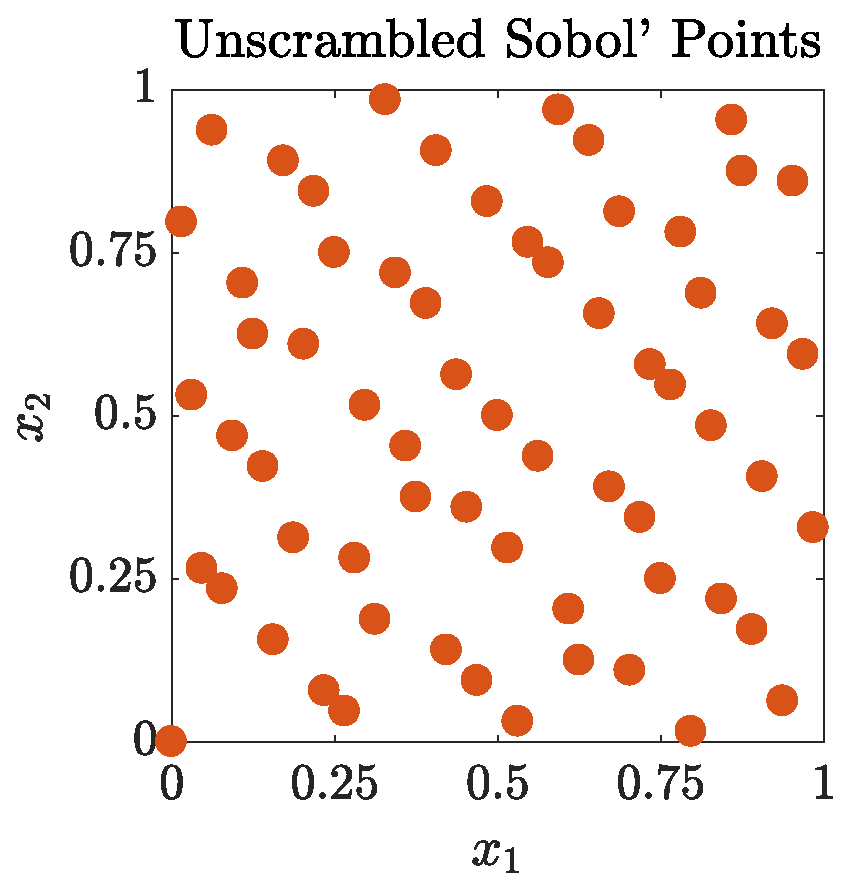
\includegraphics[height=5cm]{figures/USobolPoints}
	%\end{figure}
	\begin{figure}[htp]
		\centering
		\begin{subfigure}[b]{0.48\textwidth}
			\includegraphics[width=\textwidth]{../figures/IIDPoints}
			\caption{IID}
		\end{subfigure}
		\centering
		\begin{subfigure}[b]{0.48\textwidth}
			\includegraphics[width=\textwidth]{../figures/SSobolPoints}
			\caption{Scrambled Sobol'}
		\end{subfigure}
	\end{figure}
\end{frame}












\subsection{Walsh Kernels}

\begin{frame}{Walsh Kernels}

The Walsh covariance kernels are of the form
% Consider the covariance kernels of the form,
\begin{align}
\label{eqn:digital_shift_in_kernel}
C_{\vtheta}(\vx, \vt) = K_{\vtheta} (\vx \ominus \vt)
\end{align}
where $\ominus$ is bitwise subtraction and 
\begin{align}
\label{eqn:walsh_kernel}
K_{\vtheta} (\vx \ominus \vt) =  
\prod_{\ell=1}^d  1 + \eta_\ell \omega_{r} (x_\ell \ominus t_\ell), \quad \veta = (\eta_1, \cdots, \eta_d), \quad \vtheta = (r, \veta)
\end{align}
where $r$ is the kernel order, $\veta$ is the kernel shape parameter.
For example, explicit expression is available for $\omega_{r}$ in the case of order $r=1$ \cite{Nuyens2013}, % and Hilbert space setup,
\begin{align}
\label{eqn:omega1}
\omega_1(x) 
% &= \prod_{l=1}^d \sum_{k=1}^\infty 
% \frac{\textup{wal}_{b,k}(x_l) }{b^{2 \lfloor \log_b k \rfloor}} 
= 6\left( \frac 16 - 2^{\lfloor \log_2 x \rfloor -1 }\right).
\end{align}
\end{frame}


\begin{frame}{Walsh Kernels}
	\vspace{-6ex}
\begin{figure}
	\centering
	\includegraphics[width=0.7\linewidth]{"../figures/walsh_kernel dim_1"}
	\caption[Walsh kernel]{Walsh kernel of order $r=1$ in dimension $d=1$. } 
	\label{fig:walshkernel-dim1}
\end{figure}
\end{frame}





\begin{frame}{Sobol' Nets and Walsh Kernels}
	

	\centering\redroundmathbox{\text{
			Walsh kernels + digital nets = \emph{$2\times 2$ block-Toeplitz} matrix
	}}
	
\end{frame}




\subsection{Fast Bayesian transform}

\iffalse
\begin{frame}{Fast Bayesian Transform}
	
	
	\begin{theorem}
		\label{thrm:hadamard_eigenvector}
		The Walsh-Hadamard matrix $\mH^{(m)}$ factorizes $\mC_{\vtheta}^{(m)}$, so that the columns of Walsh-Hadamard matrix are the eigenvectors of $\mC_{\vtheta}^{(m)}$, i.e.,
		\vspace{-2ex}
		\begin{align*}
		\mH^{(m)} \mC_{\vtheta}^{(m)}  = \mLambda^{(m)} \mH^{(m)}, \quad m \in \naturals, 
		\end{align*}
		where $(m)$ denotes the size of the matrix is $2^m \times 2^m$.
	\end{theorem}

	By this theorem
	\begin{align}
	\label{eqn:hadamard_fwht}
	\mC^{(m)} = \frac{1}{n} \mH^{(m)} \mLambda^{(m)} \mH^{(m)}, \quad \text{where} \quad \mH^{({m})} = \underbrace{ \mH^{(1)} \bigotimes \cdots \bigotimes \mH^{(1)} }_{m \; \text{times}}.
	\end{align}
\end{frame}
\fi



\begin{frame}{Fast Bayesian Transform}
	
	
	%\begin{theorem}
		%\label{thrm:hadamard_eigenvector}
		The Walsh-Hadamard matrix $\mH^{(m)}$ factorizes $\mC_{\vtheta}^{(m)}$, so that the columns of Walsh-Hadamard matrix are the eigenvectors of $\mC_{\vtheta}^{(m)}$, i.e.,
		\vspace{-2ex}
		\begin{align*}
		\mH^{(m)} \mC_{\vtheta}^{(m)}  = \mLambda^{(m)} \mH^{(m)}, \quad m \in \naturals, 
		\end{align*}
		where $(m)$ denotes the size of the matrix is $2^m \times 2^m$.
	%\end{theorem}
	
	So,
	\begin{align*}
	% \label{eqn:hadamard_fwht}
	\mC^{(m)} &= \frac{1}{n} \mH^{(m)} \mLambda^{(m)} \mH^{(m)}, \quad \text{where} \quad \mH^{({m})} = \underbrace{ \mH^{(1)} \bigotimes \cdots \bigotimes \mH^{(1)} }_{m \; \text{times}}
	\\ 
	& \text{where $\bigotimes$ is Kronecker product and }
	\mH^{(1)} =
	\begin{pmatrix}
	1 & 1 \\ 1 & -1
	\end{pmatrix}.
	\end{align*}
\end{frame}










\section{Demonstration}
















\subsection{Cancellation error}

\begin{frame}{Cancellation error in $\err_\CI$}
	\vspace{-7.5ex}
	\begin{align*}
	\err_\MLE =
	2.58\sqrt{\alert{\left( 1 - \frac{n}{\lambda_1} \right)} \,
		\frac {1}{n^2} \sum_{i=2}^{n} \frac{\abs{\ty_i}^2}{\lambda_i}  }
	,
	\quad \text{may cause cancellation error}
	\end{align*}
	\pause
	\vspace{-2ex}
	\begin{align*}
	\text{Let} \hspace{0.5cm} C_{\vtheta}(\vt, \vx) = \prod_{\ell=1}^d \left[1 + \rC_{\vtheta,\ell}(t_\ell,x_\ell) \right], \qquad  \rC_{\vtheta,\ell}:[0,1] \times [0,1] \to \reals.
	\end{align*}
	Direct computation of $\rC_{\vtheta} (\vt,\vx) = C_{\vtheta}(\vt,\vx) -1$ introduces cancellation error if the $ \rC_\ell$ are small.  So, we employ the iteration,
	\begin{align*}
	\rC_{\vtheta}^{(1)}(\vt,\vx) &= \rC_{\vtheta,1}(t_1,x_1),  \\
	\rC_{\vtheta}^{(\ell)}(\vt,\vx) &  = \rC_{\vtheta}^{(\ell-1)}[1 + \rC_{\vtheta,\ell}(t_\ell,x_\ell)] + \rC_{\vtheta,\ell}(t_\ell,x_\ell),  \hspace{1cm} \ell = 2, \ldots, d, \\
	\rC_{\vtheta}(\vt,\vx)  & = \rC_{\vtheta}^{(d)}(\vt,\vx).
	\end{align*}
	Eigenvalues of $\rmC_{\vtheta}$:  
	$(\rlambda_i)_{i=1}^n = \mV^T \rvC_1, \quad \rlambda_1 = \lambda_1 - n, \lambda_2, \ldots, \lambda_n$
	\begin{align*}
	\err_\MLE  &
	=
	\frac{2.58}{n}\sqrt{
		\frac{\rlambda_1}{\lambda_1}
		\sum_{i=2}^{n} \frac{\abs{\ty_i}^2}{\lambda_i}  
	}, 
	\hspace{0.5cm}
	\vtheta_\MLE
	&= 
	\argmin_{\vtheta}
	\left[
	\log\left(
	\sum_{i=2}^n \frac{\abs{\ty_i}^2}{\lambda_i}
	\right) 
	+ 
	\frac{1}{n}\sum_{i=1}^n \log(\lambda_i)
	\right]
	\end{align*}
	
\end{frame}










\begin{frame}[label = Problem]{Example Integrands}
	\vspace{-5ex}
	\begin{tabular}{m{8.5cm}m{2.7cm}}
		\vspace{-1ex}
		\[
		\text{Gaussian probability} =
		\int_{[\va, \vb]}
		\frac{\me^{-\vx^T\mSigma^{-1}\vx/2}}{(2\pi)^{d/2}\abs{\mSigma}^{1/2}}\,\dif\vx
		, \; \text{\smallcite{Gen93}}
		\]  & \GaussPict
		\tabularnewline [-1.2ex] \arrayrulecolor{ltred} \toprule
		\tabularnewline [-1ex]
		\uncover<2->{
			\vspace{-3ex}
			\begin{gather*}
			\text{Option pricing} =
			\int_{\reals^d}
			{
				\text{payoff}(\vx)} \,
			\underbrace{
				\frac{\me^{-\vx^T\mSigma^{-1}\vx/2}}{(2\pi)^{d/2} \abs{\mSigma}^{1/2}}}_{\text{PDF of Brownian motion at $d$ times}}\,\dif\vx, \; \text{\smallcite{Gla03}}
			\\
			\text{where} \quad \text{payoff}(\vx) =  \me^{-rT}
			\max\left(\frac 1d \sum_{k=1}^d S_k(x_k) - K, 0 \right)
			\\
			S_\ell(x_\ell) = S_0 \me^{(r -\sigma^2/2)t_\ell +
				\sigma x_\ell} =\text{stock price at time } t_\ell = \ell T/d; 
			\end{gather*}
			\vspace{-1ex}
		}
		\tabularnewline [-1.2ex] \arrayrulecolor{ltred} \toprule
		\tabularnewline [-1ex]
		\uncover<3->{
			\vspace{-3ex}
			\begin{gather*}
			\text{Keister integral}  = \int_{\mathbb{R}^d} \cos(\lVert \vx \rVert)
			\exp(-\lVert \vx \rVert^2) \,  \dvx, \quad
			d = 1, 2, \ldots \; \text{\smallcite{Kei96}}
			\end{gather*}
		}
	\end{tabular}
\end{frame}








\iffalse
\subsection{Test functions}
\frame{
\frametitle{Test functions for Numerical integration:}
\vspace{-8ex}
\begin{tabular}{m{8.5cm}m{3cm}}
{Multivariate Normal (MVN)} \vspace{-2ex}
\begin{gather*}
\mu = \int_{[\va,\vb]} \frac{\exp\bigl(- \frac 12 \vt^T \mSigma^{-1} \vt \bigr)}{\sqrt{(2 \pi)^d \det(\mSigma)}} \, \dif \vt \
\overset{\text{\smallocite{Gen93}}}{=} \
\int_{[0,1]^{d-1}} f(\vx) \, \dif \vx
\end{gather*} &
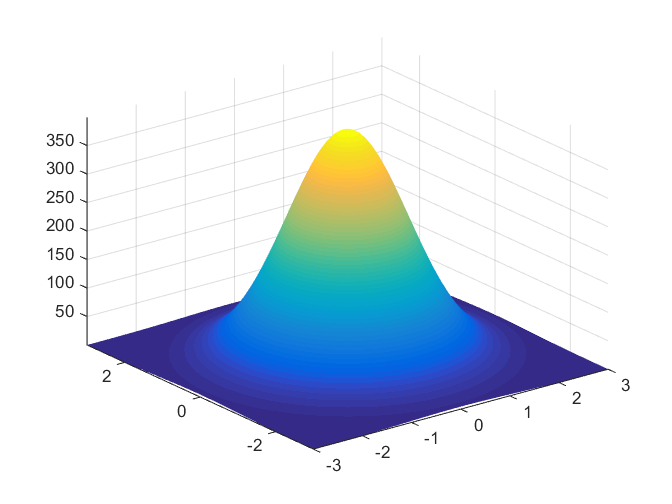
\includegraphics[width=3cm,angle=0]{../figures/Plotting_gaussian.png}
\end{tabular}
\begin{align*}
\text{Keister} &:& \mu &= \int_{\mathbb{R}^d} \cos(\lVert \boldsymbol{x} \rVert)
\exp(-\lVert \boldsymbol{x} \rVert^2) \, \mathrm{d} \boldsymbol{x},
& d = 1, 2, \ldots. & &
\\
\text{Exp(Cos)} &:& \mu &= \int_{(0,1]^d} \exp(\cos (\vx ) ) \mathrm{d} \boldsymbol{x},
& d = 1, 2, \ldots. & &
\end{align*}

}
\fi


















































\iffalse


\subsection{computation time with shift invariant kernel}
\begin{frame}
\frametitle{Computation time with Fourier kernel}
\vspace{-1ex}
\begin{figure}[htp]
\captionsetup[subfigure]{labelformat=empty}
\centering
%\begin{subfigure}[b]{0.99\textwidth}
\includegraphics[height=5cm]{zeroMean/MVN/C1sin/"MVN computeTime d_2 bernoulli_2 Period_C1sin"}
%\end{subfigure}
\caption{ MVN : d=2 r=2, C1sin }
%\label{fig:MVN_Metern_d2b2}
\end{figure}
\vspace{-3ex}
Computation time increases linearly, so we can use more than 4000 points in the Cubature, upto $2^{23}$ points with 16GB RAM computer.
\end{frame}


\fi








% \subsection{Automatic cubature}





\iffalse
\begin{frame}
\frametitle{Error bound vs actual error - Automatic cubature}
\vspace{-5ex}
\begin{figure}[htp]
\captionsetup[subfigure]{labelformat=empty}
\centering
\begin{subfigure}[b]{0.49\textwidth}
\includegraphics[height=4cm]{"AsianArithmeticMeanOption error_vs_errbd"}
\end{subfigure}
\centering
\begin{subfigure}[b]{0.49\textwidth}
\includegraphics[height=4cm]{"MVN error_vs_errbd"}
\end{subfigure}
\caption{ Left : OptionPricing, Right : MVN with various error bounds}
%\label{fig:MVN_Metern_d2b2}
\end{figure}
\vspace{-3ex}
shows the Automatic Bayesian cubature algorithm meets the error bound $\errn$.
\vspace{-3ex}
\begin{itemize}
\item
Option pricing example is only with Baker transform and Bernoulli order $r=2,4$.
\item
MVN example uses Baker, C1sin and C2sin transforms, Bernoulli order $r=2,4$ and dimension $d=2,3$.
\end{itemize}
\end{frame}
\fi


\iffalse
\begin{frame}
\frametitle{Error vs Time - Automatic cubature}
\vspace{-5ex}
\begin{figure}[htp]
\captionsetup[subfigure]{labelformat=empty}
\centering
\begin{subfigure}[b]{0.49\textwidth}
\includegraphics[height=4cm]{"AsianArithmeticMeanOption errorVtime"}
\end{subfigure}
\centering
\begin{subfigure}[b]{0.49\textwidth}
\includegraphics[height=4cm]{"MVN errorVtime 1"}
\end{subfigure}
\caption{ Left : OptionPricing $\errtol=10^{-2}$, Right : MVN $\errtol=10^{-4}$}
%\label{fig:MVN_Metern_d2b2}
\end{figure}
\vspace{-3ex}
shows the Automatic Bayesian cubature algorithms meets the specified $\errtol$ in a less than few seconds.
\vspace{-3ex}
\begin{itemize}
\item
Option pricing example is only with Baker transform and Bernoulli order $r=2,4$.
\item
MVN example uses Baker, C1sin and C2sin transforms, Bernoulli order $r=2,4$ and dimension $d=2,3$.
\end{itemize}
\end{frame}
\fi











\subsection{MVN}


\iffalse
\frame{
\frametitle{Multivariate normal probability with fixed mean $m=0$}
\vspace{-5ex}
\begin{figure}[htp]
    \centering
    \begin{subfigure}[b]{0.34\textwidth}
    \includegraphics[width=\textwidth]{zeroMean/MVN/C1sin/"MVN Error d_2 bernoulli_2 Period_C1sin"}
    \end{subfigure}
    \centering
    \begin{subfigure}[b]{0.34\textwidth}
    \includegraphics[width=\textwidth]{zeroMean/MVN/C1sin/"MVN Error d_3 bernoulli_2 Period_C1sin"}
    \end{subfigure}
    \centering
    \begin{subfigure}[b]{0.34\textwidth}
    \includegraphics[width=\textwidth]{zeroMean/MVN/C1sin/"MVN Error d_2 bernoulli_4 Period_C1sin"}
    \end{subfigure}
    \centering
    \begin{subfigure}[b]{0.34\textwidth}
    \includegraphics[width=\textwidth]{zeroMean/MVN/C1sin/"MVN Error d_3 bernoulli_4 Period_C1sin"}
    \end{subfigure}
\end{figure}
}
\fi


\frame{
\frametitle{Multivariate normal probability: Lattice }
\vspace{-5ex}
\begin{figure}[htp]
    \centering
    \begin{subfigure}[b]{0.48\textwidth}
    \includegraphics[width=\textwidth]{"../figures/Lattice/Lattice_MVN_guaranteed_time_MLE_C2sin_d2_r2_2019-Jun-27"}
    \caption{Empirical Bayes}
    \end{subfigure}
    \centering
	\begin{subfigure}[b]{0.48\textwidth}
	\includegraphics[width=\textwidth]{"../figures/Lattice/Lattice_MVN_guaranteed_time_full_C2sin_d2_r2_2019-Jun-27"}
	\caption{Full Bayes}
	\end{subfigure}
    \centering
    \begin{subfigure}[b]{0.48\textwidth}
    \includegraphics[width=\textwidth]{"../figures/Lattice/Lattice_MVN_guaranteed_time_GCV_C2sin_d2_r2_2019-Jun-27"}
    \caption{GCV}
    \end{subfigure}
% \caption{Multivariate normal probability example using 1) Empirical Bayes, 2) GCV, 3) Full Bayes stopping criterion}
\end{figure}
}




\frame{
	\frametitle{Multivariate normal probability: Sobol' }
	\vspace{-5ex}
	\begin{figure}[htp]
		\centering
		\begin{subfigure}[b]{0.48\textwidth}
			\includegraphics[width=\textwidth]{"../figures/Sobol/Sobol_MVN_guaranteed_time_MLE__d2_r1_2019-Sep-1"}
			\caption{Empirical Bayes}
		\end{subfigure}
		\centering
		\begin{subfigure}[b]{0.48\textwidth}
			\includegraphics[width=\textwidth]{"../figures/Sobol/Sobol_MVN_guaranteed_time_full__d2_r1_2019-Sep-1"}
			\caption{Full Bayes}
		\end{subfigure}
		\centering
		\begin{subfigure}[b]{0.48\textwidth}
			\includegraphics[width=\textwidth]{"../figures/Sobol/Sobol_MVN_guaranteed_time_GCV__d2_r1_2019-Sep-1"}
			\caption{GCV}
		\end{subfigure}
		\centering
		\begin{subfigure}[b]{0.48\textwidth}
			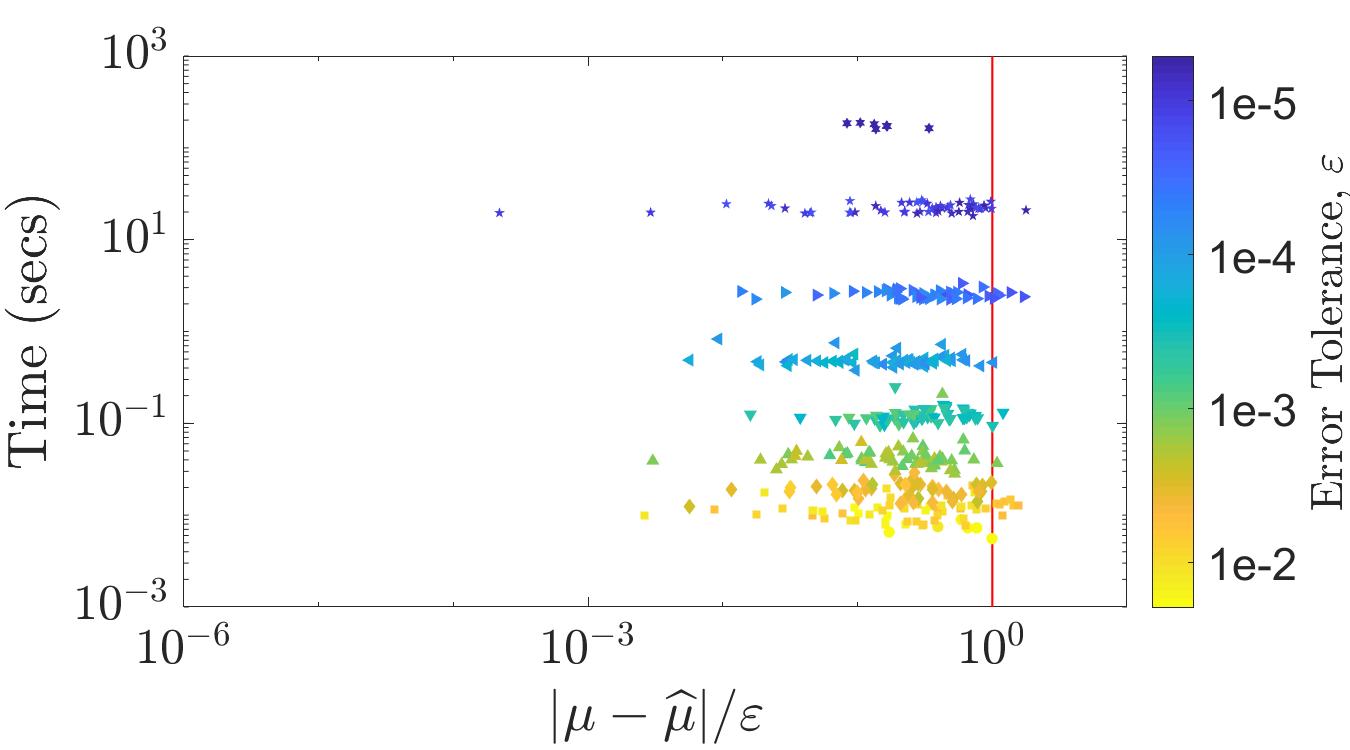
\includegraphics[height=3.25cm]{../figures/MVN_guaranteed_time_Matern_d2_2019-Jun-29}
			\caption{Slow cubature with Mat\'ern  kernel}
		\end{subfigure}	
		% \caption{Multivariate normal probability example using 1) Empirical Bayes, 2) GCV, 3) Full Bayes stopping criterion}
	\end{figure}
}





\subsection{Keister integral}


\frame{
\frametitle{Keister Integral: Lattice}
\vspace{-5ex}
\begin{figure}[htp]
	\linespread{0.7}
    \centering
    \begin{subfigure}[b]{0.43\textwidth}
    \includegraphics[width=\textwidth]{"../figures/Lattice/Lattice_Keister_guaranteed_time_MLE_C1sin_d4_r2_2019-Jun-27"}
    \caption{Empirical Bayes}
    \end{subfigure}
    \centering
	\begin{subfigure}[b]{0.43\textwidth}
	\includegraphics[width=\textwidth]{"../figures/Lattice/Lattice_Keister_guaranteed_time_full_C1sin_d4_r2_2019-Jun-27"}
	\caption{Full Bayes}
	\end{subfigure}
    \centering
    \begin{subfigure}[b]{0.43\textwidth}
    \includegraphics[width=\textwidth]{"../figures/Lattice/Lattice_Keister_guaranteed_time_GCV_C1sin_d4_r2_2019-Jun-27"}
    \caption{GCV}
    \end{subfigure}
   % \caption{Integrating Keister function using 1) Empirical Bayes, 2) GCV, 3) Full Bayes stopping criterion}
\end{figure}
}



\frame{
	\frametitle{Keister Integral: Sobol'}
	\vspace{-5ex}
	\begin{figure}[htp]
		\linespread{0.7}
		\centering
		\begin{subfigure}[b]{0.43\textwidth}
			\includegraphics[width=\textwidth]{"../figures/Sobol/Sobol_Keister_guaranteed_time_MLE__d4_r1_2019-Sep-1"}
			\caption{Empirical Bayes}
		\end{subfigure}
		\centering
		\begin{subfigure}[b]{0.43\textwidth}
			\includegraphics[width=\textwidth]{"../figures/Sobol/Sobol_Keister_guaranteed_time_full__d4_r1_2019-Sep-1"}
			\caption{Full Bayes}
		\end{subfigure}
		\centering
		\begin{subfigure}[b]{0.43\textwidth}
			\includegraphics[width=\textwidth]{"../figures/Sobol/Sobol_Keister_guaranteed_time_GCV__d4_r1_2019-Sep-1"}
			\caption{GCV}
		\end{subfigure}
		%\caption{Integrating Keister function using 1) Empirical Bayes, 2) GCV, 3) Full Bayes stopping criterion}
	\end{figure}
}



\subsection{Option pricing}

\frame{
	\frametitle{Option pricing: Lattice}
	\vspace{-5ex}
	\begin{figure}[htp]
		\linespread{0.7}
		\centering
		\begin{subfigure}[b]{0.43\textwidth}
			\includegraphics[width=\textwidth]{"../figures/Lattice/Lattice_optPrice_guaranteed_time_MLE_Baker_d12_r1_2019-Jul-9"}
			\caption{Empirical Bayes}
		\end{subfigure}
		\centering
		\begin{subfigure}[b]{0.43\textwidth}
			\includegraphics[width=\textwidth]{"../figures/Lattice/Lattice_optPrice_guaranteed_time_full_Baker_d12_r1_2019-Jul-9"}
			\caption{Full Bayes}
		\end{subfigure}
		\centering
		\begin{subfigure}[b]{0.43\textwidth}
			\includegraphics[width=\textwidth]{"../figures/Lattice/Lattice_optPrice_guaranteed_time_GCV_Baker_d12_r1_2019-Jul-8"}
			\caption{GCV}
		\end{subfigure}
		% \caption{Option pricing using 1) Empirical Bayes, 2) GCV, 3) Full Bayes stopping criterion}
	\end{figure}
}




\frame{
	\frametitle{Option pricing: Sobol'}
	\vspace{-5ex}
	\begin{figure}[htp]
		\linespread{0.7}
		\centering
		\begin{subfigure}[b]{0.43\textwidth}
			\includegraphics[width=\textwidth]{"../figures/Sobol/Sobol_optPrice_guaranteed_time_MLE__d12_r1_2019-Sep-1"}
			\caption{Empirical Bayes}
		\end{subfigure}
		\centering
		\begin{subfigure}[b]{0.43\textwidth}
			\includegraphics[width=\textwidth]{"../figures/Sobol/Sobol_optPrice_guaranteed_time_full__d12_r1_2019-Sep-1"}
			\caption{Full Bayes}
		\end{subfigure}	
		\centering
		\begin{subfigure}[b]{0.43\textwidth}
			\includegraphics[width=\textwidth]{"../figures/Sobol/Sobol_optPrice_guaranteed_time_GCV__d12_r1_2019-Sep-1"}
			\caption{GCV}
		\end{subfigure}
		% \caption{Option pricing using 1) Empirical Bayes, 2) GCV, 3) Full Bayes stopping criterion}
	\end{figure}
}






























\section{Conclusion}
\frame{\frametitle{Summary}
		\vspace{-4ex}
\begin{minipage}{\textwidth}
\linespread{1.1}
\begin{itemize}
\item Developed a \emph{technique} for a \alert{Fast Bayesian transform}
\item Developed two \alert{fast automatic Bayesian cubature} algorithms with \alert{$\Order(n\log n)$} complexity
\item Having the advantages of a kernel method and the low computation cost of Quasi Monte carlo
\item Scalable based on the complexity of the Integrand
 i.e, Kernel order and Lattice-points can be chosen to suit the smoothness of the integrand
\item Conditioning problem if the kernel $C$ is very smooth
\item Source code : \alert{\url{https://github.com/GailGithub/GAIL_Dev/tree/feature/BayesianCubature}}.
\item A part of this work was published as a paper (\ocite{JagHic09a}).
% "Fast Automatic Bayesian Cubature Using Lattice Sampling by R. Jagadeeswaran, Fred J. Hickernell" Statist. Comp., vol. 44, pp. 2559-2583, 2019. \alert{\url{ https://doi.org/10.1007/s11222-019-09895-9}}
	% (\alert{\url{https://arxiv.org/abs/1809.09803}})
\end{itemize}
\end{minipage}
}


% \section{Future work}
\frame{\frametitle{Future work}
\begin{minipage}{\textwidth}
\linespread{1.6}
\begin{itemize}
\item Choosing the \alert{kernel order $r$} and \alert{periodization} transform automatically
%\item \alert{Deterministic} interpretation of Bayesian cubature
% \item Use gradient descent to find optimal $\vtheta$
\item Diagnostics for Gaussian process assumption
\item Broaden the choice of numerical examples
\item Better handling of \alert{conditioning} problem and numerical  errors
\\
% \item Sobol pointset and Fast Walsh Transform with smooth kernels (More details next) 
\item Higher order nets and Walsh kernels could be used to achieve higher order or accuracy.
\end{itemize}
\end{minipage}
}







\frame{\frametitle{Future work : More applications}
\vspace{-4ex}
\begin{itemize}
\item \alert{Control variates} : 
We would like to approximate a function of the form
$ (f - \beta_1 g_1 -, ... , - \beta_p g_p) $, then
\begin{align*}
f = \mathcal{N} \left( \beta_0 + \beta_1 g_1 + , ... , + \beta_p g_p, s^2 \mCtheta  \right)
\end{align*}
\item \alert{Function approximation} : 
consider approximating a function of the form
\begin{align*}
\int_{[0,1]^d} \underbrace{ f(\vphi(\vt)) . \abs{\frac{\partial \vphi}{\partial \vt}} }_{g(\vt)} \dvt,&
\quad 
\text{where $\abs{\frac{\partial \vphi}{\partial \vt}}$ is Jacobian, then}&
\\
g(\vpsi(\vx)) = f( \underbrace{ \vphi(\vpsi(\vx) }_{\vx } ) .& \abs{\frac{\partial \vphi}{\partial \vt} }  (\vpsi(\vx)),
\quad
f(\vx) = g(\vpsi(\vx)) . \frac{1}{  \abs{\frac{\partial \vphi}{\partial \vt}}  (\vpsi(\vx)) }
\end{align*}
Finally, the function approximation is
\begin{align*}
\tilde{f}(\vx) &= \tilde{g}(\vpsi( \vx )) = \sum w_i C(.,.)
\end{align*}
\end{itemize}
}

\iffalse

\frame{
\frametitle{Low discrepancy points}
\vspace{-5ex}
\begin{figure}[htp]
    \centering
    \begin{subfigure}[b]{0.35\textwidth}
    \includegraphics[width=\textwidth]{figures/IIDPoints}
    \end{subfigure}
    \centering
    \begin{subfigure}[b]{0.35\textwidth}
    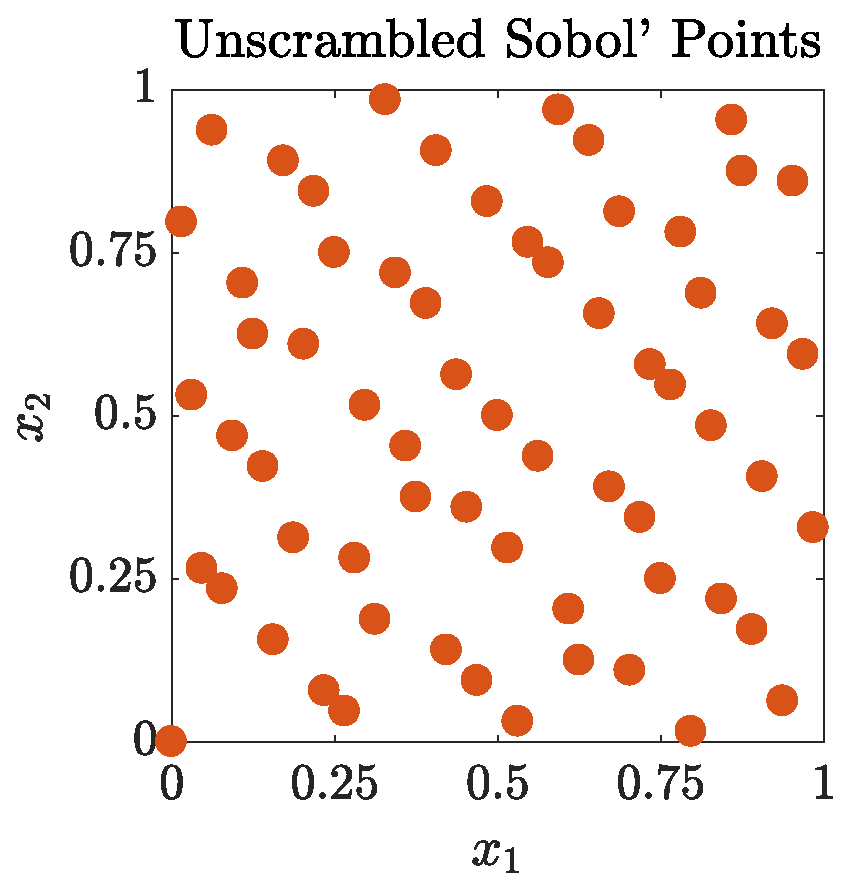
\includegraphics[width=\textwidth]{figures/USobolPoints}
    \end{subfigure}
    \centering
    \begin{subfigure}[b]{0.35\textwidth}
    \includegraphics[width=\textwidth]{figures/SSobolPoints}
    \end{subfigure}
    \centering
    \begin{subfigure}[b]{0.35\textwidth}
    \includegraphics[width=\textwidth]{figures/ShiftedLatticePoints}
    \end{subfigure}
\end{figure}
}
\fi

%\thankyouframe

\begin{frame}[plain,c]
%\frametitle{A first slide}

\begin{center}
\Huge Thank you!
%\item Thank you GAIL friends
\end{center}

\end{frame}






\appendix





% \subsection{Full Bayes}

\begin{frame}
	\frametitle{Parameter estimation - Full Bayes}
	\vspace*{-6ex}
	Treat $m$ and $s$ as hyper-parameters with a non-informative, conjugate prior, namely $\vrho_{m,s^2}(\xi, \lambda) \propto 1/\lambda$.
	Then the posterior density for the integral $\mu$ given the data is
	\vspace*{-2.0ex}
	\begin{align*}
	\rho_{\mu}(z | \vf = \vy) 
	%& \propto \int_{0}^\infty \int_{-\infty}^\infty \rho_{\mu}(z | \vf = \vy, m = \xi, s^2 = \lambda)  
	% \rho_{\vf}(\vy | \xi, \lambda ) \rho_{m, s^2}(\xi, \lambda) \, \D \xi \D \lambda \\
	& \propto \left(1 +  \frac{1}{n-1} \frac{(z - \mu_{\full})^2}{\widehat{\sigma}_{\full}^2} \right)^{-n/2}
	\end{align*}
	\pause
	\vspace{-4ex}
	\begin{align*}
	\text{Where} \;
	\\
	\mu_{\full} &= \mu_\MLE
	\\
	\hsigma^2_{\full} 
	& = \frac{1}{n-1}
	\vy^T\left[ \mCthetaInv 
	- \frac{ \mCthetaInv \vone\vone^T \mCthetaInv}{\vone^T \mCthetaInv \vone}  \right]\vy
	\times  \left[\frac{(1 - \vc^T \mCthetaInv \vone)^2}{\vone^T \mCthetaInv \vone} + (c_0  -\vc ^T \mCthetaInv \vc) \right]
	\\ &\mathbb{P}_f \left[ |\mu-\hmu_{\full}|  \leq \err_{\full} \right]  = 99\%,
	\\ \err_{\full} &:= t_{n-1,0.995} \hat{\sigma}_{\full} > \err_{\MLE}
	\end{align*}
\end{frame}
























% \subsection{GCV}

\begin{frame}
	\frametitle{Parameter estimation - Generalized Cross validation}
	\vspace*{-5ex}
	Let $\ty_i = \Ex[f(\vx_i ) | \vf_{-i} = \vy_{-i}]$.
	The cross-validation criterion, which is to be minimized, is sum of squares of the difference between these conditional expectations and the observed values: :
	\vspace*{-2.0ex}
	\begin{align*}
	%\textup{CV} &= \sum_{i=1}^n (y_i - \ty_i)^2 = \sum_{i=1}^n \left(\frac{\zeta_i }{a_{ii}} \right)^2, \quad 
	\text{Let}\; \bm{\zeta} &= \mCthetaInv(\vy - m \vone), 
	% \\
	% & \qquad 
	\qquad a_{ii} \; \text{the diagonal elems of} \; \mCthetaInv = \begin{pmatrix} a_{ii}  & \vA_{-i,i}^T \\  \vA_{-i,i} & \mA_{-i,-i}\end{pmatrix}
	\\
	\GCV &
	= \frac{\sum_{i=1}^n\zeta_i^2}{\left(\frac 1n \sum_{i=1}^n a_{ii} \right)^2} 
	= \frac{(\vy - m\vone)^T \mCtheta^{-2} (\vy - m \vone)}{\left(\frac 1n \trace(\mCthetaInv) \right)^2}.
	\end{align*}
	\pause
	\vspace{-2ex}
	\begin{align*}
	\vtheta_{\GCV} &= \argmin_{\vtheta} \left\{\log \left(  \vy^T \left[\mCtheta^{\alert{-2}} - \frac{\mCtheta^{\alert{-2}} \vone \vone^T \mCtheta^{\alert{-2}}}{\vone^T \mCtheta^{\alert{-2}} \vone}  \right] \vy \right)  
	- 2 \log \left ( \trace(\mCthetaInv) \right ) \right\}
	\\
	% s^2_{\GCV} & : = \vy^T \left[\mCtheta^{-2} - \frac{\mCtheta^{-2} \vone \vone^T \mCtheta^{-2}}{\vone^T \mCtheta^{-2} \vone}  \right] \vy  \left[ \trace(\mCthetaInv) \right]^{-1}, 
	% \quad m_{\GCV} := \frac{\vone^T \mCtheta^{-2} \vy}{\vone^T \mCtheta^{-2} \vone}. 
	\intertext{The credible interval width, $\err_{\MLE}$, is given by}
	\err_{\GCV} & = 2.58 \; s_{\GCV} \; \sqrt{c_{0,\vtheta} - \vc_{\vtheta}^T\mCthetaInv\vc_{\vtheta} }
	\end{align*}
\end{frame}



\section{General Prior}



\begin{frame}
	\frametitle{Parameter estimation - Full Bayes - General prior}
	\vspace*{-6ex}
	What if $\vrho_{m,s^2}(\xi, \lambda) \; \propto \; g( 1/\lambda )$ ?
	
	\begin{align*}
	{\rho_{\mu}(z | \vf = \vy)} & \propto \mathcal{LT} \{ g(1/\cdot) \}^{(\frac{n-4}2)} \left(\chi \right) \\
	& \propto
	\mathcal{LT} \left\{ g({1}/{\cdot})
	\right\}^{(\frac{n-4}2)} \left( 1 +  \frac{(z - \hmu_{\textup{full}})^2}{(n-1)\widehat{\sigma}_{\textup{full}}^2}\right) \quad % \text{by} \quad \eqref{eqn:full_bayes_student_short}.
	\end{align*}
	Thus, $\rho_{\mu}(z | \vf = \vy)$  is proportional to $\left(\frac{n-4}{2}\right)$th derivative of the Laplace transform of $g(1/\cdot)$ evaluated at $\chi$, where $\chi \propto { 1 +  \frac{(z - \hmu_{\textup{full}})^2}{(n-1)\widehat{\sigma}_{\textup{full}}^2} } $.
	
	Our motivation to experiment with the general prior was to show that it may
	be possible to infer the prior from the integrand samples.
\end{frame}






\section{Periodization}



\begin{frame}{Periodization Transforms}
	\vspace*{-5ex}
	Suppose the original integral is \vspace*{-1ex}
	\begin{equation*}
	\mu := \int_{(\va,\vb)^d} g(\vt) \, \dif \vt, \hspace{0.2cm}
	\text{where $g$ is smooth}, \text{not periodic. }
	\end{equation*}
	The Baker's transform, the tent transform, \vspace*{-1ex}
	\begin{align*} % \label{eq:bakerTrans}
	\vPsi: \vx \mapsto (\Psi(x_1),  \ldots, \Psi(x_d)),  \quad \Psi(x)  =1 - 2 \abs{x - 1/2}, \quad f(\vx) = g(\vPsi(\vx)).
	\end{align*} \pause
	% allows us to write $\mu$ in the form of \eqref{eqn:defn_mu}, where $f(\vx) = g(\vPsi(\vx))$. 
	% Since  $\Psi'(x)$ is not continuous, $f$ does not have continuous derivatives. 
	A family of smoother variable transforms: \vspace*{-3ex}
	% that can also preserve continuity of derivatives from the original integrand $g$ takes the form
	%\begin{subequations} %\label{eq:varTrans}
	\begin{align*}
	\vPsi: \vx \mapsto (\Psi(x_1),  \ldots, \Psi(x_d)), \quad \Psi:[0,1] \mapsto [0,1], \hspace{0.2cm}
	%\end{align*}
	%This allows us to write $\mu$ in the form of \eqref{eqn:defn_mu} with
	%\begin{align*}
	f(\vx) = g(\vPsi(\vx)) \prod_{\ell = 1}^d \Psi'(x_\ell).
	\end{align*}
	% \end{subequations}
	% for $r \in \natzero$, if the following hold:
	% then $f$ has continuous, periodic mixed partial derivatives of up to order $r$ in each direction. 
	Example: \vspace*{-2ex}
	%of this kind of transform include 
	%\cite{Sid08a}:
	\begin{align*}
	% C^0 &: \Psi(x) =  3 x^2 - 2 x^3, \quad   \Psi'(x) = 6x(1-x), \\
	C^1 & : \Psi(x) = x^3(10-15x+6x^2), \Psi'(x) = 30x^2(1-x)^2, \\
	\text{Sidi's } C^1 & : \Psi(x) = x - \frac{\sin(2\pi x)}{2 \pi}, \Psi'(x) = 1 - \cos(2\pi x),
	%\text{Sidi's } C^2 & : \Psi(x) = \frac {8 - 9 \cos(\pi x) + \cos(3 \pi x)}{16} ,   \Psi'(x) = \frac {3 \pi[3 \sin(\pi x) - \sin(3 \pi x)]}{16}, 
	\end{align*}
	when it holds
	$\Psi \in C^{r+1}[0,1]$,
	$\lim_{x \downarrow 0}x^{-r-1}\Psi'(x) = \lim_{x \uparrow 1} (1-x)^{-r-1}\Psi'(x) = 0$, and 
	$g \in C^{(r, \ldots, r)}[0,1]^d$, for $r \in \natzero$.
\end{frame}



\section{Sobol'}


\begin{frame}{Walsh Transform}
	The WHT involves multiplications by $2^m \times 2^m$ Walsh-Hadamard matrices, which is constructed recursively, starting with $\mH^{(0)} = 1$,
	\begin{align}
	\nonumber
	\arraycolsep=1.4pt\def\arraystretch{0.9}
	\mH^{(1)} &=
	\begin{pmatrix}
	1 & 1 \\ 1 & -1
	\end{pmatrix}, \\
	\nonumber
	\mH^{(2)} &= 
	\begin{pmatrix}
	1 & 1 & 1 & 1 \\ 
	1 & -1 & 1 & -1 \\
	1 & 1 & -1 & -1 \\ 
	1 & -1 & -1 & 1 \\
	\end{pmatrix}, \\
	\nonumber
	& \qquad \vdots
	\\
	\label{eqn:hadamard_matrix}
	\mH^{(m)} &= 
	\begin{pmatrix}
	\mH^{(m-1)} & \mH^{(m-1)} \\ \mH^{(m-1)} & -\mH^{(m-1)}
	\end{pmatrix} 
	= \underbrace{\mH^{(1)} \bigotimes \cdots \bigotimes \mH^{(1)}}_{m \ \text{times}} 
	= \mH^{(1)} \bigotimes \mH^{(m-1)}
	\end{align}
	where $\bigotimes$ is Kronecker product.
\end{frame}






\begin{frame}{Sobol' Nets and Walsh Kernels}
	
	\begin{theorem}
		Any symmetric, positive definite, digital shift-invariant covariance kernel of the form \eqref{eqn:walsh_kernel} scaled to satisfy \eqref{addAssump}, when matched with digital net data-sites, satisfies assumptions \eqref{fastcompAssump}.  The \emph{fast Walsh-Hadamard transform} (FWHT) can be used to expedite the estimates of $\vtheta$ in \eqref{thetaSimple} and the credible interval widths \eqref{fastStoppingCriterions} in $\Order(n \log n)$ operations. The cubature, $\hmu$, is just the sample mean.
	\end{theorem}
	
	\centering\redroundmathbox{\text{
			Walsh kernels + digital nets = \emph{$2\times 2$ block-Toeplitz} matrix
	}}
	
\end{frame}





\begin{frame}{Eigenvectors of $\mCtheta$}
	\vspace{-2ex}
	The columns of Walsh-Hadamard matrix are the eigenvectors of $\mCtheta$, i.e., $\mV := \mH$
	\begin{theorem}
		\label{thrm:block-toeplitz}
		Let $\left(\vx_i\right)_{i=0}^{n-1}$ be digitally shifted Sobol' nodes and $K$ be any function,
		% positive definite kernel function such as \eqref{eqn:omega1} which matches Sobol' nodes.
		then the Gram matrix,
		\vspace{-1ex}
		$$
		\mCtheta = \bigl(C(\vx_i, \vx_j)\bigr)_{i,j=0}^{n-1} = \bigl(K(\vx_i \ominus \vx_j)\bigr)_{i,j=0}^{n-1},
		$$   
		$\text{where} \quad \quad n=2^m, \quad C(\vx, \vt) = K(\vx \ominus \vt), \quad  \vx, \vt \in [0,1)^d, \qquad
		$
		is a $2\times 2$ block-Toeplitz matrix and all the sub-blocks and their sub-sub-blocks, etc. are also $2\times 2$ block-Toeplitz. 
	\end{theorem}
	
	
\end{frame}





\begin{frame}{Iterative Computation of Walsh Transform}
	\vspace{-4ex}
	Let $\widetilde{\vy} = \mH^{(m+1)} {\vy}$ for some arbitrary $\vy \in \reals^{2n}$, $n = 2^m$. Define, 
	\begin{gather*}
	\vy = \begin{pmatrix} y_1 \\ \vdots \\ y_{2n} \end{pmatrix}, \quad 
	\vy^{(1)} = \begin{pmatrix} y_1 \\ \vdots \\ y_{n} \end{pmatrix}, \quad 
	\vy^{(2)}  = \begin{pmatrix} y_{n+1} \\ \vdots \\ y_{2n} \end{pmatrix}, \\ 
	\widetilde{\vy}^{(1)} = \mH^{(m)} \vy^{(1)} = 
	\begin{pmatrix} \widetilde{y}^{(1)}_1 \\ \widetilde{y}^{(1)}_2 \\ \vdots \\ \widetilde{y}^{(1)}_{n} \end{pmatrix}, \quad 
	\widetilde{\vy}^{(2)}  =  \mH^{(m)} \vy^{(2)} =
	\begin{pmatrix} \widetilde{y}^{(2)}_{1} \\  \widetilde{y}^{(2)}_{2} \\ \vdots \\ \widetilde{y}^{(2)}_{n} \end{pmatrix}. 
	\end{gather*}
	Then,
	\begin{align*}
	\widetilde{\vy} &= \mH^{({m+1})} {\vy} 
	= \begin{pmatrix}
	\mH^{(m)} & \mH^{(m)} \\ \mH^{(m)} & - \mH^{(m)}
	\end{pmatrix} 
	\begin{pmatrix}
	\vy^{(1)} \\ \vy^{(2)}
	\end{pmatrix}, \qquad \text{by \eqref{eqn:hadamard_matrix}} \\
	&= 
	\begin{pmatrix}
	\mH^{(m)} \vy^{(1)} + \mH^{(m)} \vy^{(2)} 
	\mH^{(m)} \vy^{(1)} - \mH^{(m)} \vy^{(2)}
	\end{pmatrix}
	= 
	\begin{pmatrix}
	\widetilde{\vy}^{(1)} + \widetilde {\vy}^{(2)} \\ 
	\widetilde {\vy}^{(1)} - \widetilde {\vy}^{(2)}
	\end{pmatrix} =: \widetilde{\vy} 
	\end{align*}
\end{frame}






\section{Credible Interval}



\begin{frame}{Cone of functions and the Credible interval}
	In this research we assume that the integrand belongs to a cone of well-behaved functions, ${\mathscr{C}}$.  
	Suppose that 
	\begin{align}
	\label{eqn:cone-homogenity}
	\abs{\mu(f) - \hmu_n(f)} \le \err_{\CI} (f(\vx_1), \cdots, f(\vx_n))
	\end{align}
	for some $f$, which it is 99\% of the time under our hypothesis. Also note that our $\err_{\CI}, \CI \in \{\MLE, \GCV\}$  % \eqref{eqn:err_MLEGCV} \eqref{FJH:eq:errFull} 
	are positively homogeneous functions, meaning, 
	\begin{align*}
	\err_{\CI} (a y_1, \cdots, a y_n) = \abs{a} \err_{\CI} ( y_1, \cdots,  y_n).
	\end{align*}
	%One can verify the homogeneity of \eqref{eqn:err_MLEGCV} and \eqref{FJH:eq:errFull} easily.
	Thus if $f$ satisfies \eqref{eqn:cone-homogenity}, then
	\begin{align*}
	\abs{\mu(af) - \hmu_n(af)} &= \abs{a} \abs{\mu(f) - \hmu_n(f)} \\
	& \le \abs{a} \err_{\textup{CI}} (f(\vx_1), \cdots, f(\vx_n) ) 
	= \err_{\textup{CI}} (a f(\vx_1), \cdots, a f(\vx_n))
	\end{align*}
	for all real $a$. Thus the set of all $f$ satisfying \eqref{eqn:cone-homogenity} is a \emph{cone}, $\mathscr{C}$. Cones of functions satisfy the property that if $f \in \mathscr{C}$ then $af \in \mathscr{C}$.
	\begin{align*}
	\mathbb{P}_f \left[
	|\mu(f)-\hmu_n(f)| \leq \err_{\CI}(f) \right] \ge 99\%.
	\end{align*}
\end{frame}











\begin{frame}{}
	\vspace{-7ex}
	Let $f_{\TRUE}(\vx) = \exp(\sum_{\ell=1}^{d} \cos(2\pi x_\ell))$ and the peaky integrand $f_{\PEAKY}(\vx) = f_{\TRUE} + a_{\PEAKY} f_{\NOISE}$, $f_{\NOISE}(\vx) = (1 - \exp(2\pi \sqrt{-1} \vx^T \vzeta))$, $\vzeta \in \reals^d$ is some $d$-dimensional vector belonging to the dual space of the lattice nodes. The $f_{\NICE}$ is obtained by kernel interpolation.
	\vspace{-4ex}
	\begin{figure}[htp]
		\centering
		\begin{subfigure}[b]{0.44\textwidth}
			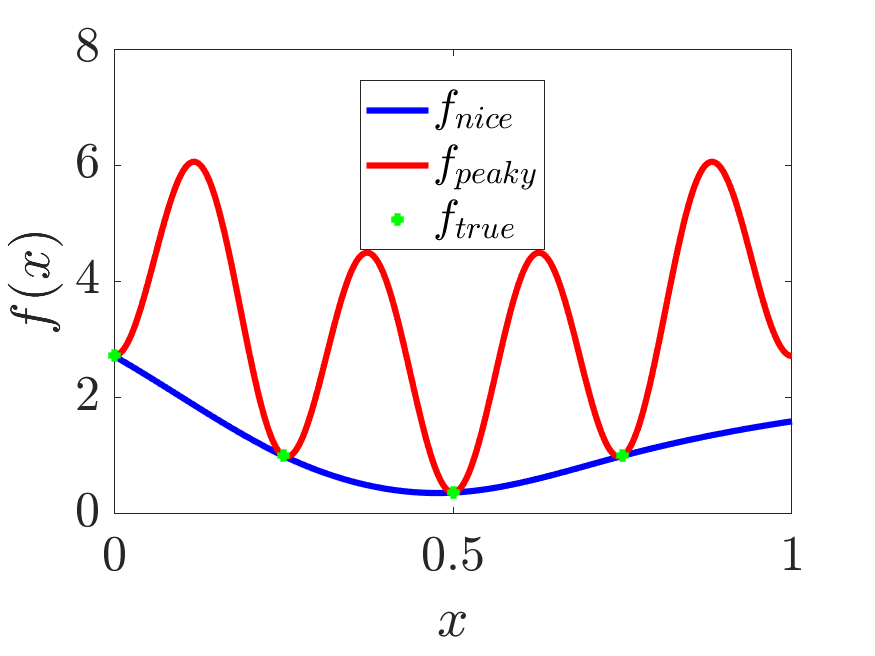
\includegraphics[width=0.9\linewidth]{../figures/cone_bayes_f_real}
		\end{subfigure}
		\centering
		\begin{subfigure}[b]{0.55\textwidth}
			\includegraphics[width=0.9\linewidth]{../figures/cone_bayes_mu_pdf}
		\end{subfigure}
		\caption{Left: Example integrands 1) $f_{\NICE}$, a smooth function, 2) $f_{\PEAKY}$, a peaky function. The function values $f_{\PEAKY}(\vx_i) = f_{\NICE}(\vx_i) = f_{\TRUE}(\vx_i) $ for $i=1, \cdots, n$. 
			Right: Probability distributions showing the relative integral position of a smooth and a peaky function. $f_{\NICE}$ lies within the center 99\% of the confidence interval, and $f_{\PEAKY}$ lies on the outside of 99\% of the confidence interval.
		}
	\end{figure}
\end{frame}









\section{Gradient Descent}

\begin{frame}{Shape parameter search using gradient descent}
	Steepest descent search is defined as:
	% as introduced in \ref{grad_descent_MLE} 
	%\eqref{Dong2017a}
	\begin{align*}
	\eta^{(j+1)}_\ell &= \eta^{(j)}_\ell - \nu \frac{\partial}{\partial \eta_\ell} \mathcal{L}_{\bm{\textup{x}}}(\vtheta | \vy), \quad j=0,1,\cdots, \quad \ell = 1, \cdots, d \\
	& \hspace{5cm} \bm{\textup{x}} \in \{\MLE, \GCV\}
	\end{align*}
	where $\nu$ is the step size for the gradient descent, $j$ is the iteration index, and $\frac{\partial}{\partial \eta_\ell} \mathcal{L}(\vtheta | \vy)$ is either \eqref{eqn:deriv_obj_func_MLE} or \eqref{eqn:deriv_obj_func_full} depending on the choice of the hyperparameter search method. The parameter $\eta_\ell$ is usually searched in the whole $\reals$ by using the simple domain transformation.
	% as explained in Section~\ref{sec:kernel_param_search}.
\end{frame}








\begin{frame}{Computing the derivative of $\mathcal{L}_{\MLE}(\vtheta | \vy)$}
	
	Taking derivative with respect to $\theta_\ell$, for $\ell=1,\cdots,d$
	\begin{align*}
	\mathcal{L}_{\MLE}(\vtheta | \vy)
	& = \log\left( {(\vy-m_\MLE\vone)^T\mCthetaInv(\vy-m_\MLE\vone)} \right) + \frac{1}{n} \log(\det(\mC_\vtheta)),
	\\
	\frac{\partial}{\partial \theta_\ell} \mathcal{L}_{\MLE}(\vtheta | \vy)
	& = - \frac
	{\left((\vy-m_\MLE\vone)^T\mCthetaInv\right)^T 
		\left( \frac{\partial \mC}{\partial \theta_\ell} \right)
		((\vy-m_\MLE\vone)^T\mCthetaInv)}
	{(\vy-m_\MLE\vone)^T\mCthetaInv(\vy-m_\MLE\vone)}
	\\ & \qquad
	+ \frac 1n \trace{\left( \mCthetaInv \frac{\partial \mC}{\partial \theta_\ell} \right)}
	, \quad \text{where} \quad m_\MLE = \frac{\vone^T \mCthetaInv \vy }{ \vone^T \mCthetaInv \vone}, 
	\end{align*}
	where we used some of the results from \smallcite{Dong2017a}.  After using the fast Bayesian transform properties
	\begin{align}
	\label{eqn:deriv_obj_func_MLE}
	\frac{\partial}{\partial \theta_\ell} \mathcal{L}_{\MLE}(\vtheta | \vy)
	&=  \frac 1n \sum_{i=1}^{n} \frac{\bar{\lambda}_{i(\ell)}}{\lambda_i}
	- \left({ \sum_{i=2}^n \frac{\abs{\tvy_i}^2 \bar{\lambda}_{i(\ell)}}{\lambda_i^2}}\right)
	\left( {\sum_{i=2}^n \frac{\abs{\tvy_i}^2}{\lambda_\ell}} \right)^{-1}
	\end{align}
	
\end{frame}








\begin{frame}{Computing the derivative of $\mathcal{L}_{\GCV}(\vtheta | \vy)$}
	
	
	Similarly for the generalized cross-validation
	\begin{align*}
	\mathcal{L}_{\GCV}(\vtheta | \vy) &= \log \left(  \vy^T \left[\mC^{-2}_\vtheta - \frac{\mC^{-2}_\vtheta \vone \vone^T \mC^{-2}_\vtheta}{\vone^T \mC^{-2}_\vtheta \vone}  \right] \vy \right)  
	- \log \left ( \trace(\mC^{-2}_\vtheta) \right ), 
	\\
	%\mathcal{L}_{\GCV}(\vtheta | \vy) &= \log \left( {(\vy-m_\MLE\vone)^T\mC^{-2}_\vtheta(\vy-m_\MLE\vone)} \right)  
	% - \log \left ( \trace(\mC^{-2}_\vtheta) \right ), 
	%\\
	%\frac{\partial}{\partial \theta_\ell}  \mathcal{L}_\GCV(\vtheta | \vy)
	%&= \left ( \sum_{i=2}^n \frac{\abs{\widetilde{y}_i}^2}{\lambda_i^2} \right)^{-1}
	% \frac{\partial}{\partial \theta_\ell} \left ( \sum_{i=2}^n \frac{\abs{\widetilde{y}_i}^2}{\lambda_i^2} \right)
	% -2 \left( \sum_{i=1}^n \frac{1}{\lambda_i} \right)^{-1}
	% \frac{\partial}{\partial \theta_\ell} \left( \sum_{i=1}^n \frac{1}{\lambda_i} \right),
	% \\
	& \qquad \text{where} \quad m_{\GCV} = \frac{\vone^T \mC_\vtheta^{-2} \vy}{\vone^T \mC_\vtheta^{-2} \vone},
	\end{align*}
	After using the fast Bayesian transform properties
	\begin{align}
	\nonumber
	\frac{\partial}{\partial \theta_\ell}  \mathcal{L}_\GCV(\vtheta | \vy)
	& = -2 \left ( \sum_{i=2}^n \frac{\abs{\widetilde{y}_i}^2}{\lambda_i^2} \right)^{-1}
	\left ( \sum_{i=2}^n \frac{\abs{\widetilde{y}_i}^2 \bar{\lambda}_{i(\ell)} }{\lambda_i^3}    \right) \\
	\label{eqn:deriv_obj_func_full}	
	& \hspace{2cm}
	+ 2 \left( \sum_{i=1}^n \frac{1}{\lambda_i} \right)^{-1}
	\left( \sum_{i=1}^n \frac{\bar{\lambda}_{i(\ell)} }{\lambda_i^2}  \right),
	\end{align}
	where $\bar{\lambda}_{i(\ell)}$ is the derivative of the $i$th eigenvalue of the Gram matrix, $\mC$, in the $\ell$th variable.
\end{frame}















\begin{frame}{Product Kernels}
	\vspace{-3ex}
	Product kernels in $d$ dimensions are of the form,
	\begin{align}
	\label{eqn:prod_kernel}
	C_{\vtheta}(\vt, \vx) = 
	\prod_{\ell=1}^d \biggl[ 1 - \eta_\ell \; \mathfrak{C}(x_\ell,t_\ell) \biggr]
	\end{align}
	where $\eta_\ell$ is called shape parameter.
	
	Derivative of the product kernel when $\eta_1=\cdots=\eta_d=\eta$
	\begin{align*}
	\frac{\partial}{\partial \eta} C_{\vtheta}(\vt, \vx) = ({d}/{\eta} ) C_{\vtheta}(\vt, \vx) 
	\biggl(
	1 - 
	\frac{1}{d} \sum_{\ell=1}^d
	\frac{1}
	{ 1 - \eta \mathfrak{C}(x_\ell,t_\ell) }
	\biggr).
	\end{align*}
	
	When $\eta_\ell$ is different for each $\ell = 1,\cdots,d$
	\begin{align*}
	\frac{\partial}{\partial \eta_\ell} C_{\vtheta}(\vt, \vx) = \frac{1}{\eta_\ell} 
	{ C_{\vtheta}(\vt, \vx) }
	\biggl(
	1 - 
	\frac{1}
	{ 1 - \eta_\ell \mathfrak{C}(x_\ell,t_\ell) }
	\biggr).
	\end{align*}
\end{frame}








\begin{frame}{To compute $\bar{\lambda}_{i(\ell)}$}
	If $\mV$ does not depend on $\vtheta$ then one can fast compute the derivative of Gram matrix $\mC$,
	\begin{align}
	\nonumber
	\displaystyle \frac{\partial \mC}{\partial \theta_\ell} 
	& = \frac 1n \mV \frac{\partial {\mLambda}}{\partial \theta_\ell} \mV^H
	= \frac 1n \mV \bar{\mLambda}_{(\ell)} \mV^H, \quad
	\text{using} \quad  \mC = \frac 1n \mV \mLambda \mV^H
	\\
	\nonumber
	& \text{where} \quad \bar{\mLambda}_{(\ell)} = \diag(\bar{\vlambda}_{(\ell)}), \quad \text{and}
	\\
	\label{eqn:deriv_eigenval_gram_matrix}
	&  \quad \bar{\vlambda}_{(\ell)} = \frac{\partial \vlambda}{\partial \theta_\ell} = \left( \frac{\partial \lambda_i}{\partial \theta_\ell} \right)_{i=1}^n 
	= \left( \frac{\partial }{\partial \theta_\ell} \mV^H {\vC_1} \right)
	= \mV^H \left( \frac{\partial }{\partial \theta_\ell} {C_\vtheta(\vx_1,\vx_i)} \right)_{i=1}^n,
	\end{align}
	where we used the fast Bayesian transform property $\vlambda = \mV^H C_1$. %\eqref{eqn:fast_transform_to_eigvalues}.
\end{frame}












\begin{frame}[allowframebreaks]
	\frametitle{References}
	\bibliographystyle{IEEEtran}
	\bibliography{../FJH22,../FJHown22}{}
	% \bibliography{../FJHown23}{}	
	%\bibliography{../mybib}{}
\end{frame}

\end{document}
